% main.tex
\documentclass[a4paper,12pt,twoside]{report}
\usepackage{hydroNova}

\begin{document}
\justifying
\selectlanguage{french}

%----------------------------------------------------------------
% PAGES PRÉLIMINAIRES
%----------------------------------------------------------------
\pagestyle{preStyle}
\pagenumbering{roman}

% PAGE DE GARDE
\begin{titlepage}
  \begin{center}
    \begin{minipage}{0.45\textwidth}
      \begin{flushleft}
        
\includegraphics[height=3.5cm]{public/isetlogo.png}
      \end{flushleft}
    \end{minipage}
    \hfill
    \begin{minipage}{0.45\textwidth}
      \begin{flushright}
        
\includegraphics[height=3.5cm]{public/logosociete.jpeg}
      \end{flushright}
    \end{minipage}
    
    \vspace{1.5cm}
    {\fontsize{14}{17}\selectfont\textbf{Institut Supérieur des Études Technologiques de Mahdia}}\\[0.3cm]
    {\fontsize{12}{15}\selectfont\textbf{Département : Technologies de l'Informatique}}\\[0.3cm]
    {\fontsize{12}{15}\selectfont\textbf{Développement des Systèmes d'Information}}\\[1.5cm]
    
    \rule{\linewidth}{0.6pt} \\[1cm]
    {\fontsize{22}{26}\selectfont\textbf{Rapport de Projet de Fin d'Études}}\\[0.8cm]
    \rule{\linewidth}{0.6pt} \\[2cm]
    
    {\fontsize{18}{22}\selectfont\textbf{HydroNova : Serre Intelligente et Automatisée}}\\[0.4cm]
    {\fontsize{14}{17}\selectfont\textbf{IoT · Intelligence Artificielle · Application Mobile}}\\[2.5cm]
    
    \begin{minipage}[t]{0.45\textwidth}
      \begin{flushleft}
        \textbf{Élaboré par :}\\[0.2cm]
        Wael Houidi\\[0.1cm]
        Ahmed Melien
      \end{flushleft}
    \end{minipage}
    \hfill
    \begin{minipage}[t]{0.45\textwidth}
      \begin{flushright}
        \textbf{Encadré par :}\\[0.2cm]
        Mme. Afifa KHALIFA (Académique)\\[0.1cm]
        M. Hamza SESSI (Entreprise)
      \end{flushright}
    \end{minipage}
    
    \vfill
    {\fontsize{12}{15}\selectfont\textbf{Organisme d'Accueil :} MicroEdition}\\[0.4cm]
    {\fontsize{12}{15}\selectfont\textbf{Période :} 02 Février 2026 -- 01 Juin 2026}\\[0.4cm]
    \vspace*{0.5cm}
  \end{center}
\end{titlepage}

% RÉSUMÉ
\clearpage
\thispagestyle{preStyle}
\begin{center}
  {\fontsize{14}{17}\selectfont\bfseries Résumé}
\end{center}
\noindent
Ce rapport présente le projet \textbf{HydroNova}, une solution de serre intelligente et automatisée dédiée à la production de fourrage hydroponique. Conçu pour répondre à la pénurie mondiale d'eau et à l'instabilité climatique, ce système permet de réduire la consommation d'eau de près de 90\% par rapport aux méthodes agricoles traditionnelles~\cite{hydroponics_water}.

L'architecture du système repose sur une infrastructure multi-couches découplée : une couche Internet des Objets (IoT) pilotée par un contrôleur Edge Raspberry Pi assurant une régulation environnementale autonome ; une couche d'Intelligence Artificielle utilisant des réseaux de neurones convolutifs (CNN) quantifiés pour la détection en temps réel des maladies végétales ; et un noyau backend sous Spring Boot exploitant TimescaleDB pour l'ingestion de données temporelles. L'interaction utilisateur est assurée par une application mobile Flutter pour l'agriculteur et un tableau de bord React/Grafana pour la supervision administrative. Développé selon la méthodologie du Cycle en V, ce projet valide l'intégration entre le matériel embarqué et l'architecture logicielle cloud.

\noindent\textbf{Mots-clés :} Hydroponie, IoT, Raspberry Pi, Intelligence Artificielle, CNN, Flutter, MQTT, Cycle en V, Agriculture 4.0.

\vspace{1cm}
\selectlanguage{english}
\begin{center}
  {\fontsize{14}{17}\selectfont\bfseries Abstract}
\end{center}
\noindent
This report presents the HydroNova project, an intelligent and automated greenhouse solution dedicated to hydroponic fodder production. Designed to address global water scarcity and climate variability, the system reduces water consumption by up to 90\% compared to traditional agricultural methods.

The system architecture is built upon a decoupled multi-layered infrastructure: an Internet of Things (IoT) layer featuring a Raspberry Pi edge controller ensuring autonomous environmental regulation; an Artificial Intelligence layer utilizing quantized CNN architectures for real-time plant disease detection; and a Spring Boot backend leveraging TimescaleDB for temporal data ingestion. User interaction is provided through a Flutter mobile application for farmers and a React/Grafana dashboard for administrative supervision. Developed following the V-Model engineering methodology, this project validates the integration between embedded hardware and cloud software architecture.

\noindent\textbf{Keywords:} Hydroponics, IoT, Raspberry Pi, Artificial Intelligence, CNN, Flutter, MQTT, V-Model, Agriculture 4.0.
\selectlanguage{french}

% DÉDICACES WAEL
\clearpage
\thispagestyle{preStyle}
\null\vspace*{\fill}
\begin{center}
  {\fontsize{26}{30}\selectfont\bfseries DÉDICACES}\\[1cm]
  \rule{0.5\textwidth}{0.5pt}\\[1.5cm]
\end{center}
\begin{flushright}
  \itshape
  Je dédie ce travail à ma famille, les piliers silencieux de ma force. Merci pour votre soutien inconditionnel, vos immenses sacrifices et pour avoir cru en moi tout au long de mon parcours académique.\\[0.5cm]
  
  À ma mère, Moufida Mighri, la pierre angulaire de ma réussite et ma première et plus grande supportrice. Ton amour et tes prières ont été la lumière me guidant à travers chaque défi. J'espère que cet accomplissement te rend fière.\\[0.5cm]
  
  À l'âme de mon défunt oncle, Amor Mighri. Bien que tu ne sois plus parmi nous, ta mémoire reste une part indélébile de mon parcours, et ton nom reste gravé dans mon cœur comme une source d'inspiration constante.\\[0.5cm]
  
  À mes encadrants, pour leurs conseils inestimables, leur patience et l'expertise technique qui a permis de forger ce projet.\\[0.5cm]
  
  Enfin, à tous ceux qui ont contribué, ne serait-ce que par un mot gentil, à l'aboutissement de ce travail.\\[0.8cm]
  
  \textbf{\Large Wael HOUIDI}
\end{flushright}
\vspace*{\fill}

% DÉDICACES AHMED
\clearpage
\thispagestyle{preStyle}
\null\vspace*{\fill}
\begin{center}
  {\fontsize{26}{30}\selectfont\bfseries DÉDICACES}\\[1cm]
  \rule{0.5\textwidth}{0.5pt}\\[1.5cm]
\end{center}
\begin{flushright}
  \itshape
  À ma famille,\\
  pour leur soutien inconditionnel et leurs immenses sacrifices\\
  tout au long de mon parcours académique.\\[0.5cm]
  
  À mes encadrants,\\
  pour leurs directives, leur patience et leur précieuse expertise technique.\\[0.5cm]
  
  \textbf{\Large Ahmed MILIEN}
\end{flushright}
\vspace*{\fill}

% REMERCIEMENTS
\clearpage
\thispagestyle{preStyle}
\begin{center}
  {\fontsize{16}{20}\selectfont\bfseries Remerciements}
\end{center}
\noindent
Avant tout, nous rendons grâce à \textbf{Allah Le Tout-Puissant} de nous avoir accordé la santé, la patience, la volonté et le courage nécessaires pour mener à bien ce projet de fin d'études. C'est par Sa grâce et Sa bénédiction que ce travail a pu voir le jour.

\noindent
Nous tenons ensuite à exprimer notre profonde et sincère gratitude à toutes les personnes qui ont contribué, de près ou de loin, à la réalisation de ce projet.

\noindent
Nos plus vifs remerciements s'adressent à notre encadrante académique, \textbf{Mme. Afifa Khalifa}, pour la qualité de son encadrement, ses orientations pertinentes, sa disponibilité constante et son suivi rigoureux tout au long de l'élaboration de ce rapport. Ses conseils avisés ont été déterminants pour garantir la rigueur scientifique de notre travail.

\noindent
Notre sincère reconnaissance va également à notre encadrant professionnel, \textbf{M. Hamza Sessi}, pour sa confiance, son accompagnement technique et le partage généreux de son expertise. Nous remercions aussi l'ensemble de l'équipe de \textbf{MicroEdition} pour leur accueil chaleureux et la mise à disposition des ressources matérielles et logicielles indispensables à la concrétisation de ce projet.

\noindent
Nous adressons nos remerciements respectueux aux membres du jury pour l'honneur qu'ils nous font en acceptant d'évaluer ce travail.

\noindent
Nous exprimons également notre gratitude envers l'administration et le corps professoral de l'\textbf{ISET de Mahdia}, en particulier le Département Technologies de l'Informatique, pour la qualité de la formation dispensée et pour nous avoir transmis les fondements académiques nécessaires à notre parcours.

\noindent
Enfin, une pensée particulière va à nos familles, pour leur soutien inconditionnel et leurs sacrifices constants, ainsi qu'à nos amis et collègues pour leur encouragement et leur présence à nos côtés tout au long de cette expérience enrichissante.

% TABLE DES MATIÈRES, FIGURES, TABLEAUX, ACRONYMES
\clearpage
\thispagestyle{preStyle}
\tableofcontents

\clearpage
\thispagestyle{preStyle}
\listoffigures

\clearpage
\thispagestyle{preStyle}
\listoftables

% ACRONYMES
\clearpage
\thispagestyle{preStyle}
\begin{center}
  {\fontsize{16}{20}\selectfont\bfseries LISTE DES ACRONYMES}\\[0.4cm]
  \rule{0.5\textwidth}{0.5pt}
\end{center}
\begin{center}
\renewcommand{\arraystretch}{1.6}
\begin{tabularx}{\textwidth}{@{} p{3.5cm} X @{}}
  \rowcolor[HTML]{2C3E50}
  \textcolor{white}{\textbf{Acronyme}} & \textcolor{white}{\textbf{Signification}} \\
  \rowcolor[HTML]{EFEFEF}
  \textbf{AI / IA}      & Artificial Intelligence / Intelligence Artificielle \\
  \textbf{API}          & Application Programming Interface \\
  \rowcolor[HTML]{EFEFEF}
  \textbf{CNN}          & Convolutional Neural Network (Réseau de Neurones Convolutif) \\
  \textbf{CRISP-DM}     & Cross Industry Standard Process for Data Mining \\
  \rowcolor[HTML]{EFEFEF}
  \textbf{DES}          & Dynamic Ensemble Selection \\
  \textbf{Edge AI}      & Intelligence Artificielle embarquée en périphérie réseau \\
  \rowcolor[HTML]{EFEFEF}
  \textbf{F1-Score}     & Moyenne harmonique entre précision et rappel \\
  \textbf{HTTP / HTTPS} & HyperText Transfer Protocol / Secure \\
  \rowcolor[HTML]{EFEFEF}
  \textbf{IoT}          & Internet of Things (Internet des Objets) \\
  \textbf{JWT}          & JSON Web Token \\
  \rowcolor[HTML]{EFEFEF}
  \textbf{LLM}          & Large Language Model \\
  \textbf{META-DES}     & Meta-learning for Dynamic Ensemble Selection \\
  \rowcolor[HTML]{EFEFEF}
  \textbf{MQTT / MQTTS} & Message Queuing Telemetry Transport / Secure \\
  \textbf{NLP}          & Natural Language Processing (Traitement du Langage Naturel) \\
  \rowcolor[HTML]{EFEFEF}
  \textbf{ONNX}         & Open Neural Network Exchange \\
  \textbf{ORM}          & Object-Relational Mapping \\
  \rowcolor[HTML]{EFEFEF}
  \textbf{RAG}          & Retrieval-Augmented Generation \\
  \textbf{REST}         & Representational State Transfer \\
  \rowcolor[HTML]{EFEFEF}
  \textbf{SDK}          & Software Development Kit \\
  \textbf{SSL / TLS}    & Secure Sockets Layer / Transport Layer Security \\
  \rowcolor[HTML]{EFEFEF}
  \textbf{UI / UX}      & User Interface / User Experience \\
  \rowcolor[HTML]{EFEFEF}
  \textbf{UML}          & Unified Modeling Language \\
  \textbf{VLM}          & Vision Language Model \\
  \rowcolor[HTML]{EFEFEF}
  \textbf{VQA}          & Visual Question Answering \\
  \textbf{WIP}          & Work In Progress \\
  \rowcolor[HTML]{EFEFEF}
  \textbf{WS / WSS}     & WebSocket / WebSocket Secure \\
\end{tabularx}
\end{center}
\addcontentsline{toc}{chapter}{Liste des Acronymes}

%----------------------------------------------------------------
% DÉBUT DE LA NUMÉROTATION ARABE
%----------------------------------------------------------------
\clearpage
\pagestyle{mainStyle}
\pagenumbering{arabic}
\setcounter{page}{1}

%----------------------------------------------------------------
% INCLUSION DES CHAPITRES
%----------------------------------------------------------------
\chapter*{Introduction Générale}
\addcontentsline{toc}{chapter}{Introduction Générale}
\markboth{Introduction Générale}{Introduction Générale}

Le secteur agricole se trouve actuellement confronté à une convergence de défis mondiaux. Le changement climatique, la dégradation des écosystèmes et la pénurie croissante d'eau douce remettent en question les paradigmes agricoles traditionnels. Simultanément, la croissance de la population mondiale exige des rendements supérieurs sur des terres arables en diminution constante. Dans ce contexte, l'agriculture en environnement contrôlé, et plus particulièrement la production de fourrage hydroponique, émerge comme une alternative viable et efficiente. En substituant le sol par des solutions aquatiques recirculantes et riches en nutriments, les systèmes hydroponiques peuvent réduire la consommation d'eau agricole jusqu'à 90~\% selon la littérature~\cite{hydroponics_water}, tout en augmentant significativement la densité de production par mètre carré.

Cependant, la vulnérabilité intrinsèque des systèmes hydroponiques représente un défi d'ingénierie majeur. Dépourvus de la capacité de tamponnement naturel du sol, les environnements agricoles en intérieur exigent une précision microclimatique élevée. Même des fluctuations transitoires de l'humidité ambiante, de la température, des cycles photopériodiques ou de la conductivité électrique des nutriments peuvent déclencher une défaillance des cultures. De plus, les conditions denses et humides nécessaires à la croissance du fourrage favorisent la propagation fongique. Par conséquent, la supervision humaine manuelle se révèle insuffisante pour répondre aux exigences en temps réel de l'hydroponie moderne.

Ce projet de fin d'études, mené sous la supervision technique de \textbf{MicroEdition}, répond à ce dilemme à travers la conception architecturale et l'implémentation du système \textbf{HydroNova}. Cette plateforme constitue un écosystème agricole intelligent et autonome qui articule l'ingénierie matérielle et l'analyse logicielle. En faisant converger l'Internet des Objets (IoT) pour une régulation environnementale déterministe, et l'Intelligence Artificielle (Edge AI) pour des diagnostics biologiques proactifs, le système vise à réduire significativement l'intervention humaine dans la boucle de contrôle agricole.

La problématique centrale qui motive ce projet est la suivante : \textit{Comment concevoir un système de contrôle IoT résilient et capable de fonctionner hors-ligne, augmenté par des réseaux de neurones convolutifs embarqués, afin d'automatiser, superviser et protéger biologiquement la production de fourrage hydroponique ?}

Pour aborder cette question avec méthode, ce rapport est structuré en quatre chapitres détaillés :
%%%%%%A corriger
\begin{itemize}
  \item \textbf{Chapitre I} établit le contexte général du projet, présente l'organisme d'accueil (MicroEdition), effectue une analyse des solutions agricoles existantes, et définit l'architecture globale proposée ainsi que la méthodologie en Cycle en V adoptée.
  \item \textbf{Chapitre II} délimite les exigences fonctionnelles et non fonctionnelles du système, en formalisant les interactions entre les acteurs humains et matériels via les diagrammes UML (Unified Modeling Language).
  \item \textbf{Chapitre III} présente l'architecture globale du système, organisée en couches découplées, allant du réseau physique IoT (Edge) jusqu'aux couches de persistance Cloud.
  \item \textbf{Chapitre IV} couvre la réalisation technique du projet. Il détaille d'abord l'infrastructure matérielle et IoT (isolation électrique, Raspberry Pi, MQTT), puis l'intégration de l'Intelligence Artificielle embarquée (Edge AI) pour la détection des maladies. Il présente ensuite les interfaces applicatives développées (application mobile Flutter et tableau de bord web React), pour conclure sur la stratégie de déploiement Cloud (Docker, TimescaleDB, Spring Boot) et l'orchestration du backend.
\end{itemize}
\chapter{Cadre Général du Projet}
	
	\section*{Introduction}
	\addcontentsline{toc}{section}{Introduction}
	
Ce chapitre pose les fondements contextuels indispensables à la compréhension de la portée et des ambitions du HydroNova. Il s'ouvre sur la présentation de MicroEdition, l'organisme d'accueil, en détaillant son positionnement stratégique dans le domaine de l'intelligence embarquée et des écosystèmes IoT industriels. Nous procédons ensuite à une analyse critique du paysage technologique agricole actuel, en identifiant les lacunes structurelles des solutions disponibles sur le marché. Cette analyse nous permet de justifier la pertinence et la valeur ajoutée de notre système proposé. Le chapitre s'achève par la présentation de la méthodologie en Cycle en V, cadre d'ingénierie retenu pour structurer l'ensemble du processus de développement et de validation.
	
	%----------------------------------------------------------------
	\section{Présentation de l'organisme d'accueil}
	%----------------------------------------------------------------
	
	\subsection{Profil de l'entreprise et vision stratégique}
	
Fondée en 2025 et implantée au sein de la Pépinière d'Entreprises de Mahdia, MicroEdition est une entreprise technologique  spécialisée dans les Technologies de l'Information et de la Communication. Sa vocation fondatrice est de combler le fossé entre la recherche académique avancée et les solutions industrielles directement déployables sur le terrain.
L'intégration au sein de la pépinière offre à l'entreprise un écosystème collaboratif particulièrement stimulant: accès à une infrastructure technique adaptée au prototypage rapide, à un réseau interdisciplinaire de partenaires académiques et industriels, et à un environnement propice à l'expérimentation à moindre risque. Cette proximité avec la recherche constitue un atout déterminant pour mener des projets à forte composante d'innovation, comme le HydroNova.
	
	\subsectiontitle{Piliers technologiques centraux}
	
	Le portefeuille opérationnel de MicroEdition s'articule autour de trois domaines d'expertise profondément interconnectés :
	
	\begin{itemize}
		\item \textbf{Ingénierie Logicielle: } L'entreprise conçoit des architectures logicielles modulaires et évolutives, ainsi que des interfaces utilisateurs multiplateformes et réactives. L'accent est mis sur la maintenabilité, la testabilité et la scalabilité des systèmes produits, afin de garantir une évolution fluide et durable des solutions développées.
		
		\item \textbf{Internet des Objets Industriel (IIoT): } MicroEdition développe des réseaux embarqués résilients capables d'orchestrer des interactions matérielles autonomes. Ces réseaux s'appuient sur des protocoles de communication légers et sur des processus déterministes, garantissant la fiabilité des échanges même dans des environnements contraints en bande passante ou soumis à des coupures réseau fréquentes.
		
		\item \textbf{Intelligence Artificielle Embarquée (Edge AI): } Le déploiement de modèles de Machine Learning directement sur des dispositifs à ressources limitées constitue la compétence différenciante de l'entreprise. Cette approche dite Edge-first élimine la latence et les risques d'indisponibilité inhérents à l'inférence basée sur le Cloud, tout en préservant la confidentialité des données produites localement.
	\end{itemize}
	\subsectiontitle{Dynamique Organisationnelle et R\&D}
	
	L'entreprise adopte une organisation hybride des processus de développement, adaptée à la nature des projets et à leurs contraintes spécifiques. Cette approche combine des cycles structurés de type prédictif pour les phases critiques, et des pratiques itératives inspirées des méthodes Agiles afin de favoriser la flexibilité, la réactivité et l'amélioration continue.
	
	La cellule dédiée à la Recherche et Développement (R\&D) est concentrée sur l'optimisation des contraintes de calcul des dispositifs "Edge" (à la périphérie du réseau). Cette compétence en R\&D a été un facteur déterminant pour le système \textit{HydroNova}, fournissant l'expertise requise pour exécuter des réseaux de neurones convolutifs directement sur un Raspberry Pi déployé localement.
	%----------------------------------------------------------------
%----------------------------------------------------------------
\section{Contexte général du projet}
%----------------------------------------------------------------

L’agriculture connaît aujourd’hui une transformation profonde sous l’effet de la révolution numérique. Face à la croissance démographique mondiale, à la raréfaction des ressources naturelles et aux changements climatiques, les méthodes agricoles traditionnelles montrent certaines limites en matière de productivité, de gestion des ressources et de résilience environnementale. Dans ce contexte, l’intégration des technologies numériques dans les systèmes agricoles apparaît comme une solution prometteuse pour améliorer l’efficacité des exploitations tout en garantissant une utilisation plus rationnelle des ressources.

Cette évolution a donné naissance au concept d’\textit{Agriculture 4.0}, qui repose sur l’exploitation des technologies de l’Internet des Objets , de l’Intelligence Artificielle , du Cloud Computing et de l’analyse des données afin de moderniser les pratiques agricoles. L’objectif est de transformer les exploitations agricoles en systèmes intelligents capables de collecter, analyser et exploiter les données en temps réel pour optimiser la prise de décision et automatiser les processus de production.

%----------------------------------------------------------------
\subsection{Agriculture intelligente et Agriculture 4.0}
%----------------------------------------------------------------

L’Agriculture 4.0 représente l’application des technologies numériques avancées au secteur agricole. Elle vise à améliorer la productivité, réduire les coûts d’exploitation et limiter l’impact environnemental des activités agricoles grâce à une gestion intelligente des ressources.

L’un des piliers fondamentaux de cette transformation est l’Internet des Objets. Les capteurs connectés permettent de mesurer en temps réel différents paramètres tels que la température, l’humidité, la luminosité, le pH ou encore la qualité de l’eau. Ces données sont ensuite transmises vers des plateformes de supervision capables de surveiller l’état des cultures et de déclencher automatiquement des actions correctives lorsque cela est nécessaire.

Parallèlement, l’Intelligence Artificielle joue un rôle croissant dans l’automatisation des tâches agricoles. Grâce aux techniques d’apprentissage automatique et de vision par ordinateur, il devient possible de détecter précocement certaines maladies végétales, d’identifier des anomalies de croissance ou encore de fournir des recommandations adaptées aux agriculteurs. Ces technologies contribuent à améliorer la qualité de la production tout en réduisant les interventions manuelles.

Enfin, les systèmes de supervision connectée offrent une visibilité globale sur l’exploitation agricole. Les données collectées par les capteurs peuvent être visualisées à travers des applications mobiles ou des interfaces web, permettant aux utilisateurs de suivre l’évolution des paramètres environnementaux, de recevoir des alertes en temps réel et de piloter les équipements à distance. Cette approche favorise une gestion plus réactive, plus précise et davantage orientée vers l’optimisation des performances.

%----------------------------------------------------------------
\subsection{Hydroponie et production de fourrage}
%----------------------------------------------------------------

Parmi les approches innovantes adoptées dans le cadre de l’agriculture intelligente, l’hydroponie occupe une place importante. Cette technique consiste à cultiver les plantes sans sol, en utilisant une solution nutritive contrôlée qui fournit directement aux racines les éléments nécessaires à leur développement. Grâce à la maîtrise des conditions de culture, l’hydroponie permet d’obtenir une croissance rapide et régulière tout au long de l’année.

Dans le domaine de l’élevage, la production de fourrage hydroponique constitue une alternative intéressante aux méthodes conventionnelles. Les graines, généralement de l’orge, sont placées dans des plateaux de culture et irriguées de manière contrôlée pendant plusieurs jours jusqu’à obtenir un tapis végétal riche en nutriments destiné à l’alimentation animale. Ce procédé permet de produire du fourrage frais en continu, indépendamment des conditions climatiques extérieures.

L’hydroponie présente plusieurs avantages significatifs. Elle permet notamment une réduction importante de la consommation d’eau, une optimisation de l’espace de production, une diminution de la dépendance aux terres agricoles ainsi qu’une meilleure maîtrise des paramètres environnementaux. De plus, la production peut être réalisée de manière continue, garantissant une disponibilité régulière du fourrage pour les exploitations d’élevage.

Cependant, cette méthode présente également certaines contraintes. Les cultures hydroponiques nécessitent un contrôle permanent des paramètres environnementaux tels que la température, l’humidité, l’éclairage et les cycles d’irrigation. Une défaillance technique ou une variation importante de ces paramètres peut affecter rapidement la qualité de la production. Par ailleurs, les environnements humides favorisent le développement de maladies et de moisissures, rendant indispensable la mise en place de mécanismes de surveillance et de détection précoce.

C’est dans cette perspective que s’inscrit notre projet, dont l’objectif est de concevoir une serre hydroponique intelligente reposant sur l’intégration de technologies IoT, d’algorithmes d’Intelligence Artificielle et d’interfaces de supervision connectées afin d’automatiser la production, d’améliorer la surveillance des cultures et d’optimiser l’utilisation des ressources.
\section{Présentation du problème}
%----------------------------------------------------------------

L’agriculture moderne fait face à de nombreux défis qui impactent directement la productivité des exploitations et la sécurité alimentaire. Dans le contexte tunisien, ces difficultés concernent aussi bien les aspects agricoles que les aspects technologiques. La mise en place d’un système hydroponique intelligent nécessite donc de répondre simultanément à ces deux catégories de contraintes.

%----------------------------------------------------------------
\subsectiontitle{Défis agricoles}
%----------------------------------------------------------------

Le secteur de l’élevage tunisien dépend fortement de la disponibilité d’un fourrage de qualité, produit de manière durable et économiquement viable. Toutefois, plusieurs facteurs limitent aujourd’hui les méthodes conventionnelles de production :

\begin{itemize}
	
	\item \textbf{Stress hydrique croissant:} La raréfaction des ressources en eau et les périodes de sécheresse récurrentes rendent l’irrigation traditionnelle de plus en plus difficile et coûteuse.
	
	\item \textbf{Coût élevé de l’alimentation animale: } Les aliments concentrés importés représentent une part importante des dépenses des éleveurs et sont fortement influencés par les fluctuations du marché international.
	
	\item \textbf{Dépendance aux conditions climatiques: } Les rendements agricoles restent fortement liés aux variations saisonnières, ce qui complique la planification de la production fourragère.
	
	\item \textbf{Risques phytosanitaires: } Les environnements humides utilisés pour la culture hydroponique favorisent l’apparition de maladies, de moisissures et d’autres agents pathogènes pouvant compromettre la qualité du fourrage.
	
	\item \textbf{Besoin d’une production continue: } Les exploitations d’élevage nécessitent un approvisionnement régulier en fourrage tout au long de l’année, indépendamment des conditions climatiques extérieures.
	
\end{itemize}

%----------------------------------------------------------------
\subsection{Défis technologiques}
%----------------------------------------------------------------

Au-delà des contraintes agronomiques liées à la production hydroponique, la conception d’une plateforme intelligente intégrant l’Internet des Objets (IoT), l’Intelligence Artificielle (IA) et les technologies Web et Mobile soulève plusieurs défis technologiques majeurs. Ces défis concernent aussi bien l’acquisition des données, l’automatisation des processus que la prise de décision intelligente.

\begin{itemize}
	
	\item \textbf{Collecte et traitement des données en temps réel: } 	
	Le système doit assurer une acquisition continue et fiable des données provenant des différents capteurs déployés dans l’environnement de culture. Les paramètres tels que la température, l’humidité, la luminosité, le niveau d’eau, le pH ou encore les cycles d’irrigation doivent être surveillés en permanence afin de garantir des conditions optimales de croissance. Cette collecte doit être accompagnée d’un traitement en temps réel permettant la détection rapide d’anomalies et la génération d’alertes pertinentes.
	
	\item \textbf{Automatisation intelligente des équipements: } 	
	La plateforme doit être capable de piloter automatiquement les différents actionneurs (pompes, électrovannes, systèmes d’éclairage, ventilateurs, etc.) en fonction des données collectées et des règles de contrôle définies. L’objectif est de réduire l’intervention humaine tout en assurant une gestion précise des ressources et un maintien optimal des conditions de culture.
	
	\item \textbf{Fonctionnement autonome et résilience du système: } 
	Dans certaines zones agricoles, les interruptions de connexion Internet peuvent être fréquentes. Le système doit donc être conçu selon une architecture capable de continuer à fonctionner localement même en mode hors ligne. Cette autonomie implique la gestion locale des données critiques, l’exécution des règles d’automatisation et la synchronisation automatique avec les services distants dès le rétablissement de la connexion.
	
	\item \textbf{Détection intelligente des maladies et des anomalies: } 
	L’identification précoce des maladies représente un enjeu majeur pour limiter les pertes de production. L’intégration de techniques de vision par ordinateur et de modèles d’apprentissage profond permet d’analyser automatiquement les images des cultures afin de détecter les symptômes de maladies, les carences nutritionnelles ou les anomalies de croissance. Le défi consiste à obtenir des modèles à la fois précis, rapides et capables de fonctionner sur des ressources matérielles limitées.
	
	\item \textbf{Supervision et contrôle à distance: } 
	Les exploitants doivent pouvoir accéder aux informations de leur installation depuis n’importe quel endroit via une interface web ou une application mobile. La plateforme doit fournir des tableaux de bord intuitifs, des visualisations en temps réel, des notifications d’alerte ainsi que des fonctionnalités de contrôle à distance garantissant une gestion efficace de l’exploitation.
	
	\item \textbf{Intégration et interopérabilité des technologies: } 
	La solution repose sur l’interaction de plusieurs composants hétérogènes: capteurs IoT, microcontrôleurs, protocoles de communication, services backend, bases de données, modèles d’intelligence artificielle, applications web et mobiles. Assurer une communication fluide, sécurisée et performante entre ces différents éléments constitue un défi essentiel pour garantir la cohérence et la fiabilité du système global.
	\item \textbf{Sécurité et protection des données: } 
	Les données collectées ainsi que les commandes de contrôle doivent être protégées contre les accès non autorisés. La mise en œuvre de mécanismes d’authentification, de chiffrement des communications et de gestion des droits d’accès est indispensable afin d’assurer la confidentialité, l’intégrité et la disponibilité des informations.
	\item \textbf{Scalabilité et évolutivité de la plateforme: } 
	La solution doit être conçue de manière modulaire afin de faciliter l’ajout de nouveaux capteurs, de nouvelles fonctionnalités ou de nouveaux modèles d’intelligence artificielle. Cette évolutivité garantit l’adaptation de la plateforme aux besoins futurs des utilisateurs et aux évolutions technologiques.
	
\end{itemize}
Face à l’ensemble de ces défis, la problématique de ce projet consiste à concevoir et développer une plateforme hydroponique intelligente capable d’automatiser la production de fourrage, d’assurer une surveillance continue des cultures et de fournir des mécanismes avancés d’aide à la décision. Cette solution doit combiner efficacement les technologies IoT, l’Intelligence Artificielle, le Cloud Computing ainsi que les applications Web et Mobile afin d’améliorer la productivité, la qualité des cultures et l’efficacité opérationnelle des exploitations agricoles modernes.
%----------------------------------------------------------------
\section{Étude de l’existant}
%----------------------------------------------------------------

\subsection{Solutions existantes}

L’analyse des solutions disponibles dans le domaine de l’agriculture intelligente révèle plusieurs plateformes hydroponiques intégrant l’automatisation, les capteurs IoT et les technologies de contrôle environnemental. Les solutions suivantes représentent des références importantes dans le secteur des systèmes agricoles intelligents. \newline

\noindent\begin{minipage}[c]{0.12\textwidth}
	\centering
	
\includegraphics[width=0.95\textwidth]{public/AgroSelf}
\end{minipage}
\hfill 
\begin{minipage}[c]{0.83\textwidth}
	\textbf{AgroSelf: } Solution hydroponique intelligente destinée à l’automatisation de la culture végétale en environnement contrôlé. Le système intègre des mécanismes de surveillance des paramètres climatiques et nutritifs afin d’optimiser la croissance des plantes tout en réduisant la consommation d’eau et d’énergie.
\end{minipage}

\vspace{1cm}  

\noindent
\begin{minipage}[c]{0.12\textwidth}
	\centering
	
\includegraphics[width=0.95\textwidth]{public/grow}
\end{minipage}
\hfill
\begin{minipage}[c]{0.83\textwidth}
	\textbf{GIY (Grow It Yourself): } Solution orientée agriculture domestique et urbaine permettant aux utilisateurs de cultiver des plantes de manière autonome. Elle propose une gestion simplifiée de l’irrigation, de l’éclairage et du suivi de croissance grâce à des technologies connectées adaptées aux petits espaces.
\end{minipage}

\vspace{1cm}  

\noindent
\begin{minipage}[c]{0.12\textwidth}
	\centering
	
\includegraphics[width=0.95\textwidth]{public/biolo}
\end{minipage}
\hfill
\begin{minipage}[c]{0.83\textwidth}
	\textbf{Biosolx: } Plateforme spécialisée dans les systèmes agricoles intelligents utilisant des capteurs et des solutions IoT pour le contrôle automatisé de l’environnement de culture. Elle vise à améliorer la productivité agricole à travers l’analyse des données en temps réel et la gestion optimisée des ressources.
\end{minipage} \newline


\subsection{Limites des solutions existantes}

Malgré les fonctionnalités avancées offertes par les solutions étudiées, plusieurs limites demeurent présentes. La plupart des solutions reposent fortement sur des infrastructures centralisées ou des services distants, ce qui peut affecter leur autonomie et leur disponibilité. Par ailleurs, les capacités d’intelligence artificielle et de diagnostic automatisé restent souvent limitées ou absentes. Certaines solutions offrent également une faible adaptabilité aux contraintes des exploitations locales et nécessitent des coûts de déploiement ou de maintenance relativement élevés. Le tableau \ref{tab:comparaison-solutions} synthétise les principales limites identifiées à travers l’analyse comparative réalisée.

\begin{table}[!htbp] 
	\centering
	\small
	\renewcommand{\arraystretch}{1.5}
	\begin{tabular}{|p{3.5cm}|p{3.5cm}|p{3.5cm}|p{3.5cm}|}
		\hline
		\rowcolor[HTML]{ECECEC} 
		\textbf{Critères} & \textbf{AgroSelf} & \textbf{GIY (Grow It)} & \textbf{Biosolx} \\ \hline
		
		\textbf{Dépendance Cloud} & Forte dépendance à une infrastructure Cloud pour le contrôle. & Fonctionnement partiellement connecté. & Architecture centralisée dépendante du système distant. \\ \hline
		
		\textbf{Intelligence du système} & Optimisation limitée aux paramètres environnementaux. & Assistance décisionnelle sans autonomie complète. & Automatisation industrielle sans intelligence contextuelle. \\ \hline
		
		\textbf{Vision et diagnostic} & Absence de détection visuelle des maladies. & Observation manuelle par l’utilisateur. & Contrôle basé uniquement sur capteurs physiques. \\ \hline
		
		\textbf{Adaptabilité locale} & Faible adaptation aux environnements ruraux. & Dépendance à la formation utilisateur. & Solution orientée industrie à grande échelle. \\ \hline
		
		\textbf{Coût et accessibilité} & Coût élevé et maintenance complexe. & Coût modéré mais dépendance au support. & Solution industrielle difficilement accessible. \\ \hline

		\textbf{Assistance agronomique} & Aucun accompagnement intelligent à l'agriculteur. & Interface passive sans conseil contextuel. & Pas d'assistance décisionnelle intégrée. \\ \hline
	\end{tabular}
	\caption{Analyse comparative des solutions hydroponiques existantes}
	\label{tab:comparaison-solutions}
\end{table}

L’étude des solutions existantes montre qu’aucune d’entre elles ne répond simultanément aux exigences suivantes : autonomie hors ligne, intégration d’une intelligence artificielle avancée pour le diagnostic biologique, et accessibilité économique adaptée au contexte agricole tunisien.

Ainsi, ces limites justifient la nécessité de proposer une nouvelle architecture plus robuste, autonome et adaptée aux contraintes locales, constituant la base du système développé dans ce projet.


	%----------------------------------------------------------------
\section{ Solution Proposée}
	%----------------------------------------------------------------
	
Pour répondre aux lacunes identifiées, nous proposons le \textbf{HydroNova} : une architecture de contrôle décentralisée et orientée \textit{Edge-first}, conçue pour garantir une résilience opérationnelle totale en mode hors-ligne, tout en tirant parti des capacités d'analyse et de supervision offertes par le Cloud lorsque la connectivité est disponible.

	La solution s'articule autour de quatre axes technologiques complémentaires, avec une priorité stratégique accordée à l'intelligence embarquée :
	
	\begin{itemize}
		\item \textbf{L’Intelligence Artificielle Embarquée (Cœur de la détection sanitaire) :} Véritable pilier de la solution, ce module repose sur un réseau de neurones convolutifs (CNN) spécifiquement entraîné pour le diagnostic phytosanitaire du fourrage hydroponique. Déployé directement sur le Raspberry Pi sous forme d'un modèle quantifié en format ONNX (FP16), il effectue une inférence locale pour identifier en temps réel les marqueurs précoces de moisissures ou de stress fongique sur les images capturées par la caméra intégrée. Le traitement s'opère intégralement en local, garantissant une latence quasi nulle et une disponibilité totale indépendante de l'état du réseau. Cette sentinelle numérique assure une vigilance sanitaire permanente, capable d'isoler une menace biologique avant même qu'elle ne soit perceptible à l'œil nu.
		
		\item \textbf{Le Contrôleur Edge Autonome (Raspberry Pi) :} Ce nœud de calcul central exécute des services multi-processus optimisés assurant la régulation déterministe du microclimat : température, hygrométrie, pH, cycles d'irrigation et éclairage artificiel. Un mécanisme de surveillance matérielle de type Watchdog garantit le redémarrage automatique de tout service défaillant, préservant ainsi l'intégrité biologique de la culture contre tout arrêt non prévu du système.
		
		\item \textbf{Backend et Gestion de Données :}  L'orchestration globale est assurée par une architecture robuste développée sous Spring Boot selon les principes de la Clean Architecture. Ce centre de commandement gère la réception asynchrone des flux télémétriques via le protocole sécurisé MQTTS, et ingère les données dans InfluxDB, une base de données spécialisée dans le stockage et l'analyse efficace des séries temporelles. Cette couche analytique transforme les relevés bruts en historiques exploitables pour l'optimisation continue des rendements. Un chatbot agronomique basé sur une architecture RAG (Retrieval-Augmented Generation) avec Gemini complète ce dispositif en offrant un accompagnement intelligent et contextualisé à l'agriculteur.
		\item \textbf{Interfaces de Supervision :}  L'interaction avec les utilisateurs est assurée par deux interfaces complémentaires. L'application mobile développée sous Flutter permet un pilotage nomade de la serre et la réception immédiate d'alertes critiques. Le tableau de bord d'administration React, associé à Grafana, offre aux gestionnaires une vue analytique haute résolution de l'ensemble du parc, avec configuration à distance et visualisation des séries temporelles.
	\end{itemize}
	En s'appuyant sur du matériel libre (Raspberry Pi) et des logiciels open-source, cette architecture réduit significativement les coûts d'acquisition et de maintenance, la rendant accessible aux exploitations de taille moyenne dans le contexte agricole tunisien. En combinant l'autonomie de l'Edge Computing aux capacités d'analyse du Cloud, cette solution vise à transformer la culture hydroponique en un processus sécurisé, intelligent et économiquement viable.
	% Positionnement de la figure immédiatement après la description

% ---------------------------------------------------------------
\section{Méthodologie de gestion de projet}
%----------------------------------------------------------------

La réussite d’un projet multidisciplinaire tel que \textit{HydroNova} repose non seulement sur les choix technologiques, mais aussi sur l’adoption d’une méthodologie de gestion adaptée à la nature hybride du système. Ce projet combine en effet plusieurs dimensions complémentaires : des composants matériels (capteurs, actionneurs, Raspberry Pi, Arduino), des communications IoT temps réel (MQTT), un module d’intelligence artificielle (inférence locale CNN, assistant VLM cloud), un backend centralisé (Spring Boot, bases de données) et des interfaces utilisateurs multiples (Flutter, React).

Le projet \textit{HydroNova} présente trois caractéristiques majeures qui justifient le recours à plusieurs méthodes:

\begin{enumerate}
	\item \textbf{Intégration matérielle et logicielle}: Le système comporte une partie embarquée critique (contrôle des actionneurs, acquisition des capteurs) qui doit respecter des contraintes de temps réel et de fiabilité. Cette partie nécessite une validation formelle et une traçabilité rigoureuse.
	\item \textbf{Développement logiciel distribué}: Le backend, l’application mobile et le tableau de bord web évoluent de manière continue. Ils appellent une gestion de flux flexible, capable de s’adapter aux changements sans bloquer l’intégration.
	\item \textbf{Module d’intelligence artificielle}: La détection des maladies repose sur des données et des modèles d’apprentissage. Ce volet exige un cycle itératif spécifique (compréhension des données, préparation, modélisation, évaluation) différent du cycle classique du génie logiciel.
\end{enumerate}

Aucune méthode unique ne couvre l’ensemble de ces exigences. Une approche méthodologique composite s’impose, où chaque sous‑système est piloté par la méthode la mieux adaptée à son domaine, le tout étant orchestré par un \textbf{cadre global en V} qui garantit la traçabilité et la cohérence d’ensemble.

%----------------------------------------------------------------
\subsection{Présentation synthétique des méthodes retenues}
%----------------------------------------------------------------

\subsubsection*{Modèle en V}
Organisé en deux branches symétriques (spécification descendante, validation ascendante), il assure une traçabilité complète entre les exigences et les tests. Chaque phase de conception est associée à une phase de vérification de même niveau. Ce modèle est particulièrement adapté aux systèmes embarqués critiques et à l’intégration matérielle.
%\begin{figure}[!htbp]
%	\centering
%	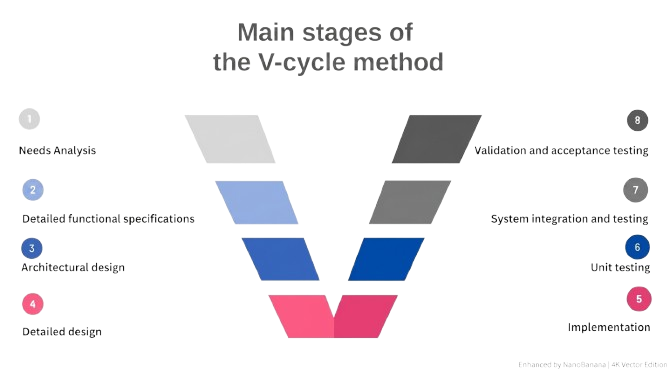
\includegraphics[width=0.75\linewidth]{public/vmodelpp}
%	\caption{Le modèle en V — phases de conception et de validation en symétrie}
%	\label{fig:vmodelpp}
%\end{figure}

\subsubsection*{Kanban}
%\begin{figure}[h!]
%	\centering	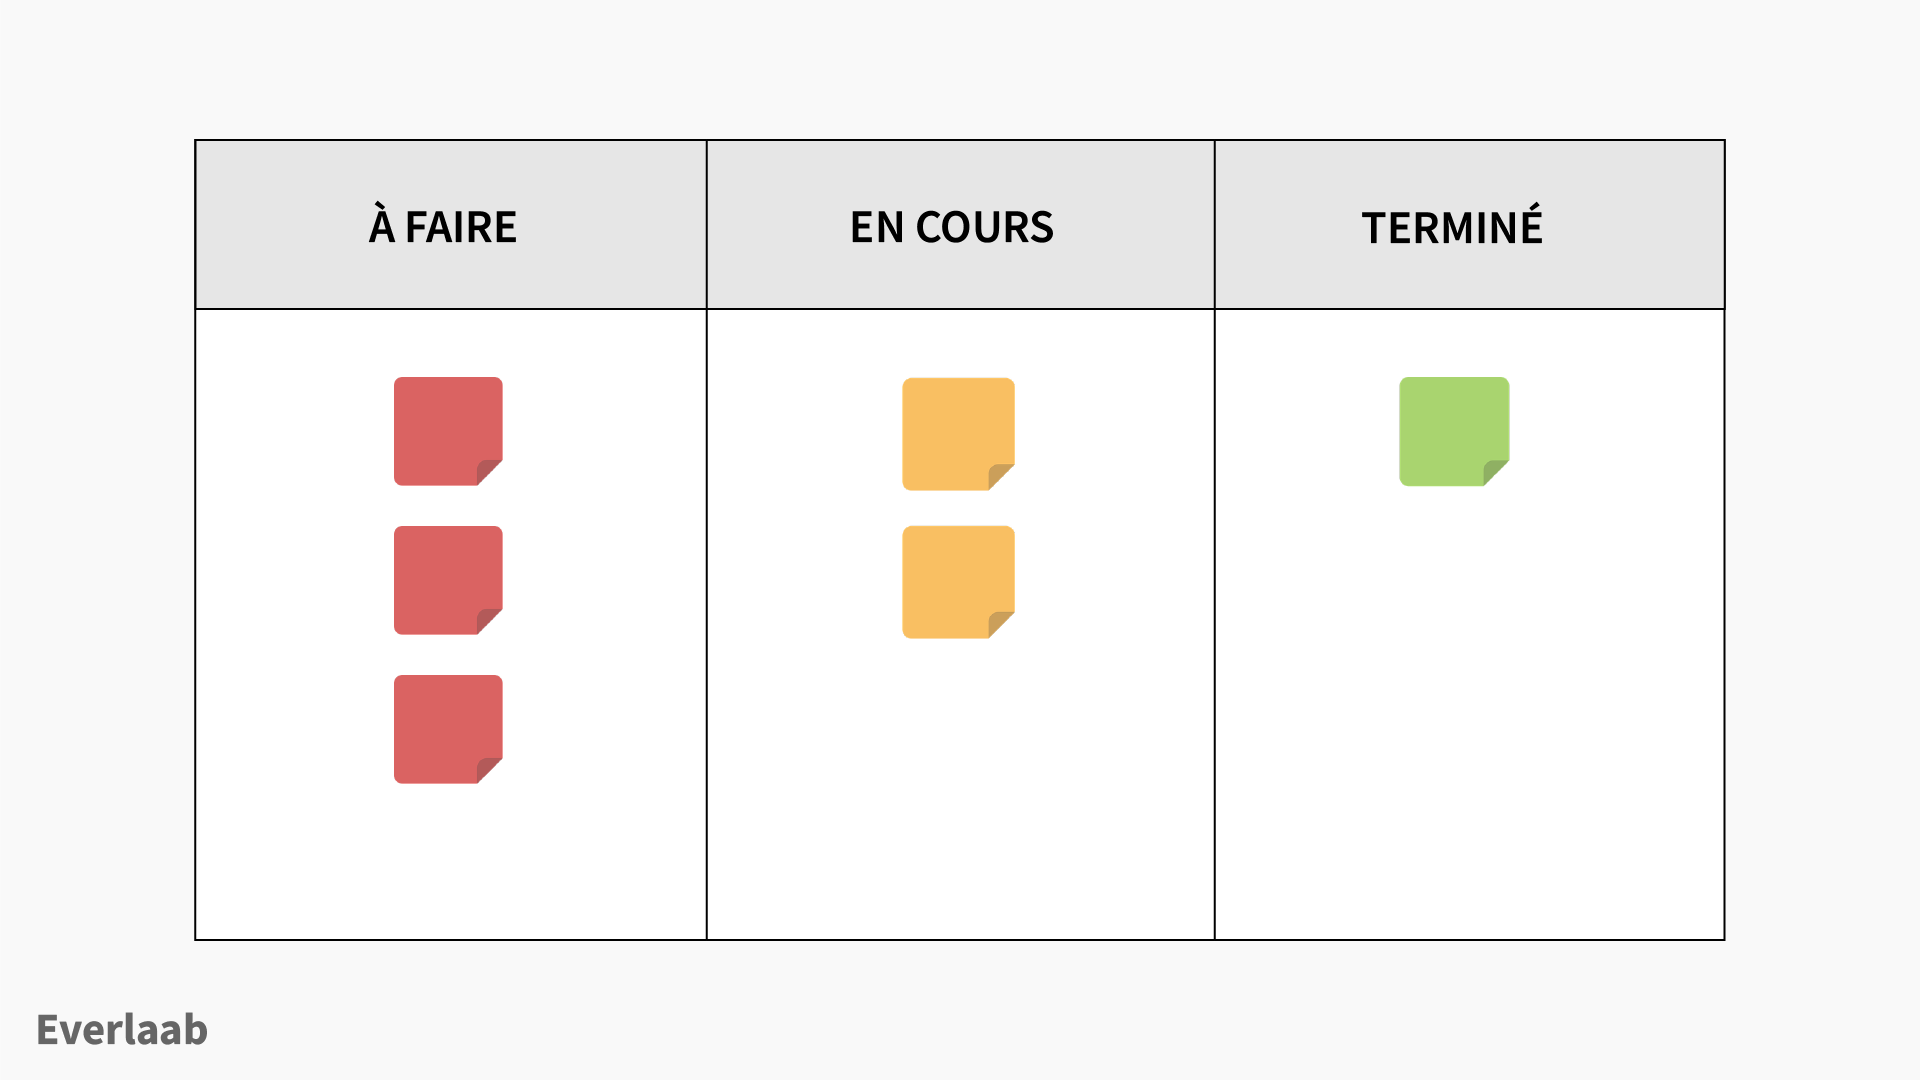
\includegraphics[width=0.75\linewidth]{public/kanban-1}
%	\caption{Fonctionnement du tableau Kanban — flux de tâches par colonnes}
%	\label{fig:kanban-1}
%\end{figure}
Méthode de gestion visuelle du travail en flux continu. Elle repose sur un tableau divisé en colonnes (À faire, En cours, Terminé) et sur une limitation du travail en cours (WIP). Kanban permet une grande flexibilité pour les tâches de développement logiciel et s’intègre facilement à d’autres cadres.


\subsubsection*{CRISP-DM}
Cadre de référence pour les projets d’intelligence artificielle. Il définit six phases itératives (compréhension du domaine, compréhension des données, préparation, modélisation, évaluation, déploiement). Ce cycle permet de revenir en arrière lorsque les résultats d’un modèle sont insuffisants.
\begin{figure}[!htbp]
	\centering
	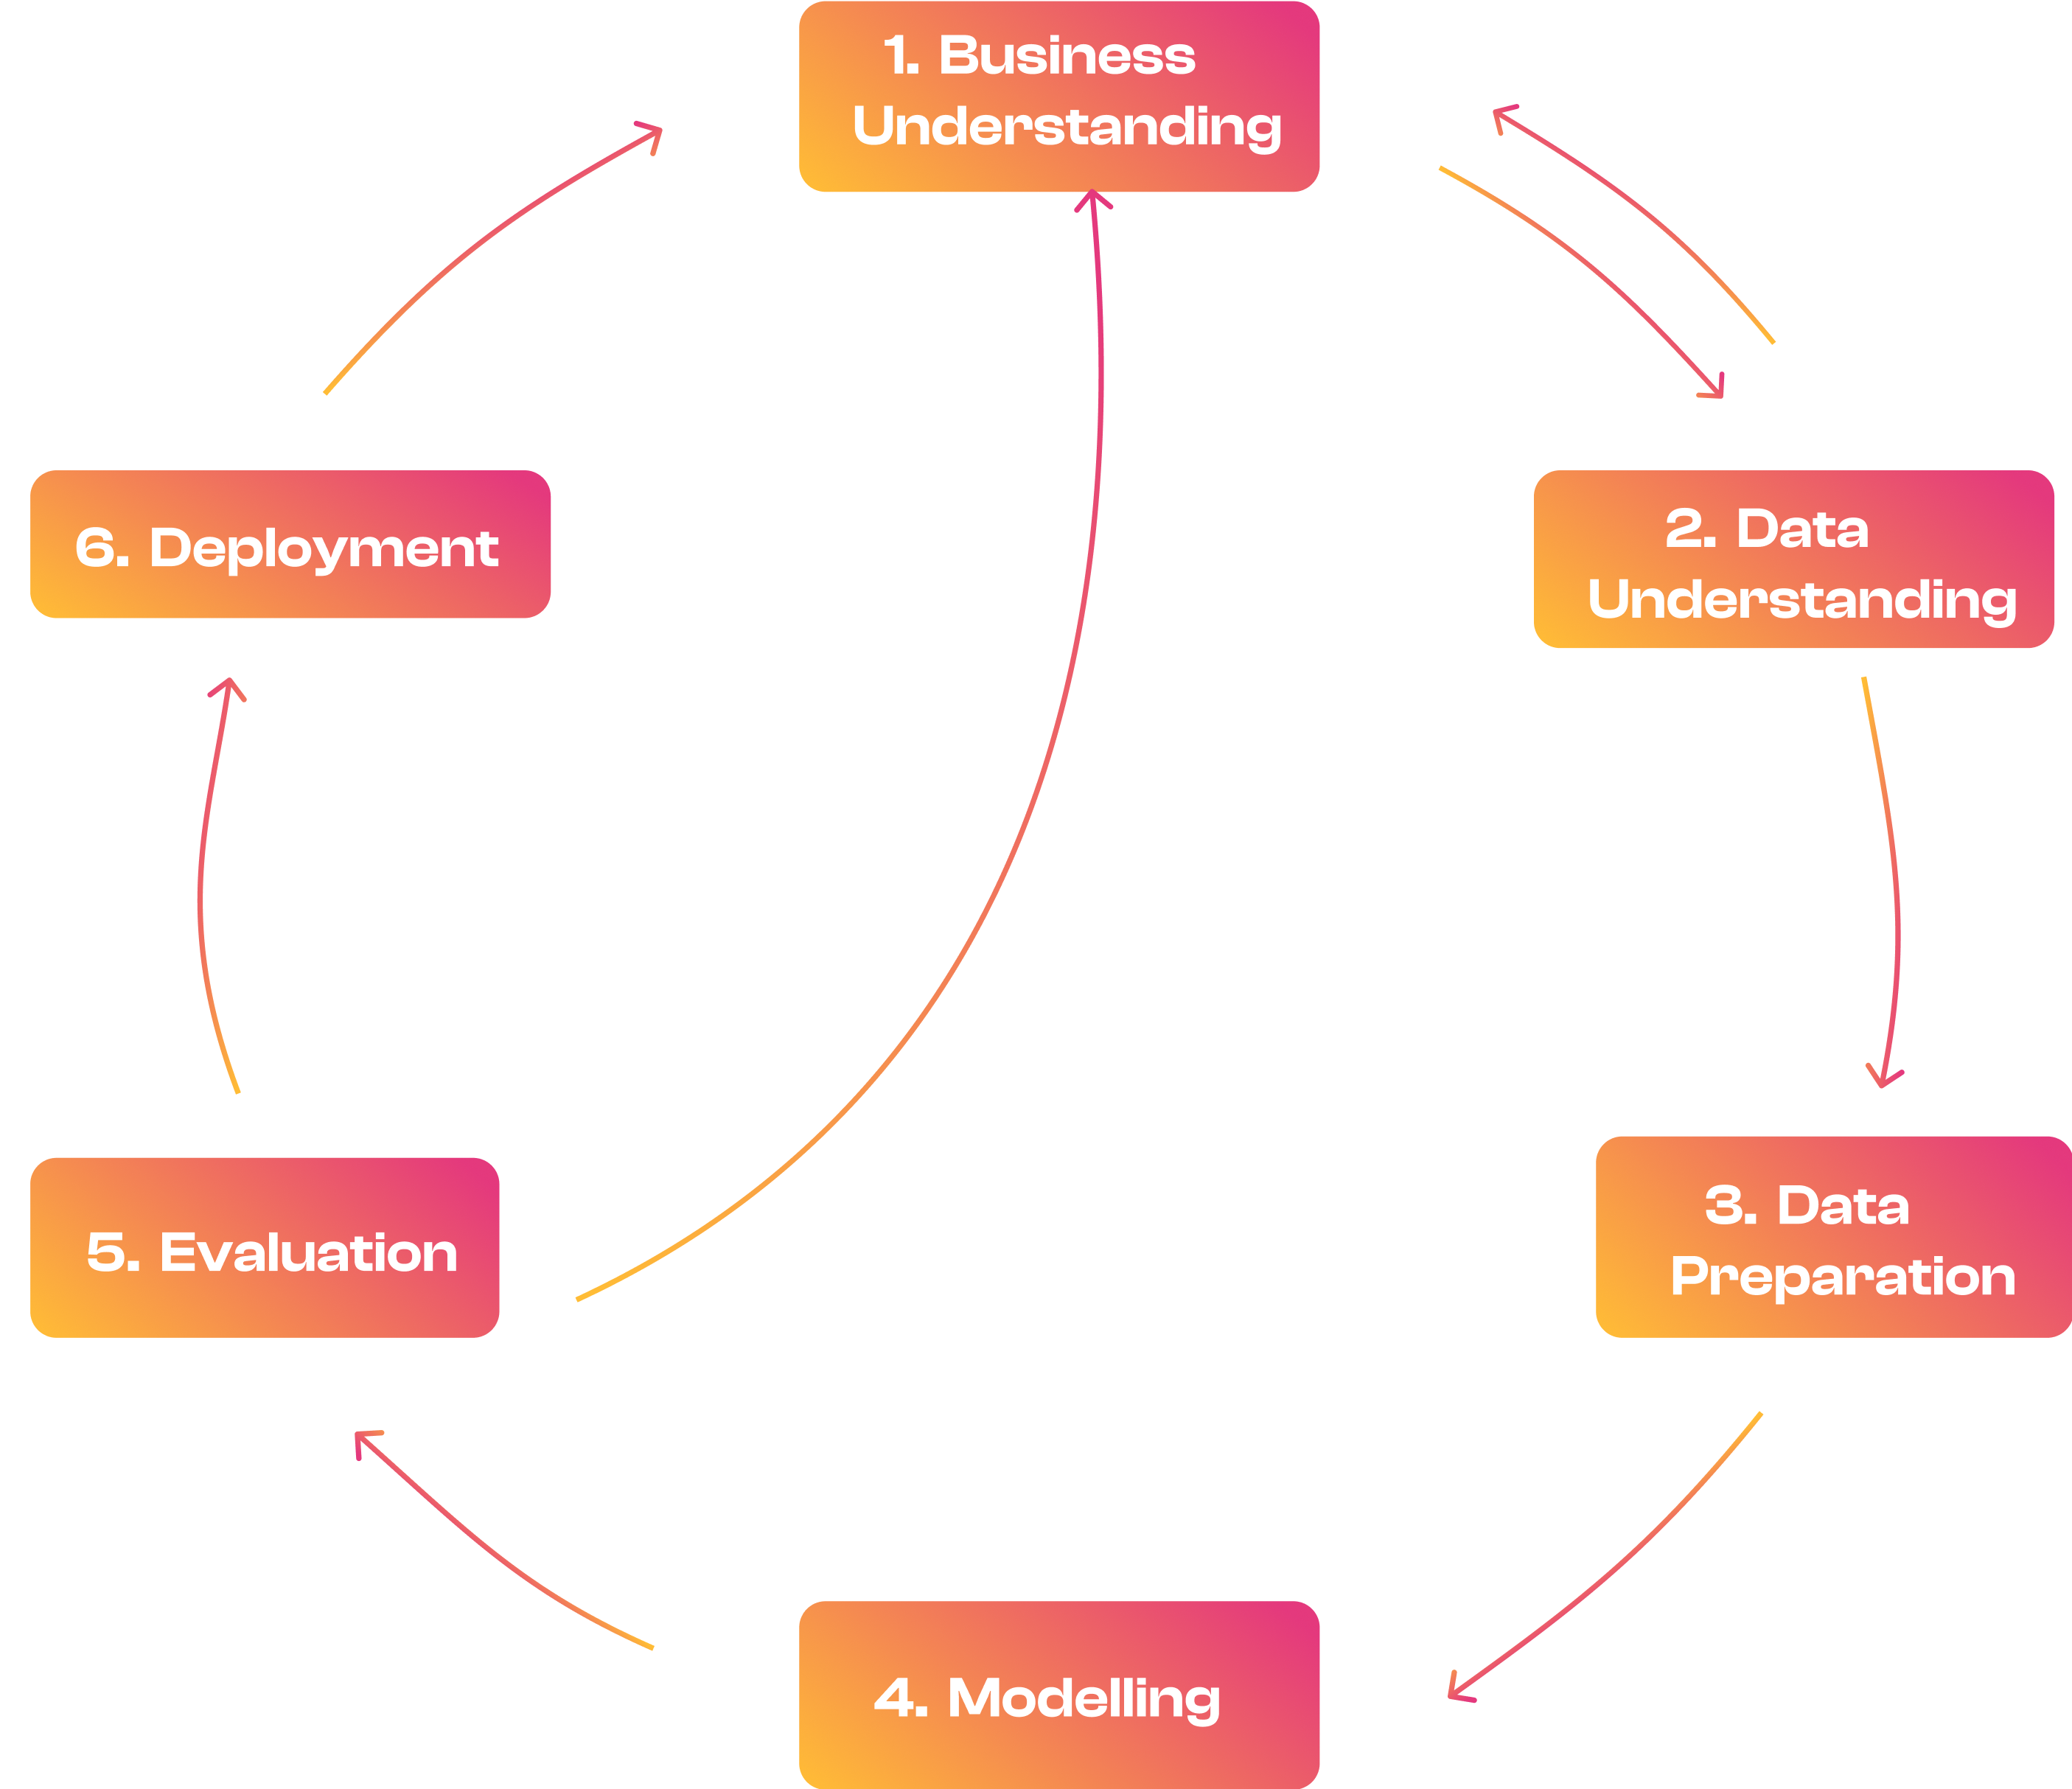
\includegraphics[width=0.6\linewidth]{public/crispdm}
	\caption{Le cycle CRISP-DM — six phases itératives pour les projets IA}
	\label{fig:crispdm}
\end{figure}

Ces trois approches présentent des profils complémentaires, comme le résume le tableau~\ref{tab:comparaison_methodologies}.

\begin{table}[!htbp]
	\centering
	\small
	\renewcommand{\arraystretch}{1.5}
	\begin{tabularx}{\textwidth}{|p{0.28\textwidth}|X|X|X|}
		\hline
		\rowcolor[HTML]{2C3E50}
		\textcolor{white}{\textbf{Critère}} & \textcolor{white}{\textbf{Kanban}} & \textcolor{white}{\textbf{Cycle en V}} & \textcolor{white}{\textbf{CRISP-DM}} \\ \hline
		\rowcolor[HTML]{EFEFEF}
		Gestion des projets IoT & Bon & Excellent & Faible \\ \hline
		Développement logiciel & Excellent & Bon & Faible \\ \hline
		\rowcolor[HTML]{EFEFEF}
		Gestion des systèmes embarqués & Moyen & Excellent & Faible \\ \hline
		Traçabilité & Moyen & Excellent & Moyen \\ \hline
		\rowcolor[HTML]{EFEFEF}
		Flexibilité & Excellent & Faible & Bon \\ \hline
		Validation formelle & Moyen & Excellent & Moyen \\ \hline
		\rowcolor[HTML]{EFEFEF}
		Projets IA & Bon & Moyen & Excellent \\ \hline
	\end{tabularx}
	\caption{Comparaison des méthodologies étudiées}
	\label{tab:comparaison_methodologies}
\end{table}

%----------------------------------------------------------------
\subsection{Hybridation au sein du modèle en V}
%----------------------------------------------------------------

Le cadre global du projet est le modèle en V. Il structure le rapport et le déroulement du projet, depuis l’analyse des besoins (chapitre III) jusqu’aux tests de validation (chapitre VI). Cependant, à l’intérieur de certaines phases du V, d’autres méthodes sont utilisées pour répondre aux spécificités des composants.

\begin{itemize}
	\item \textbf{Phase de conception détaillée}: Pour le module IA, au lieu d’une spécification linéaire, nous exécutons un cycle CRISP-DM complet (compréhension des données, préparation, modélisation, évaluation). Ce cycle est itéré localement jusqu’à l’obtention d’un modèle satisfaisant. Une fois figé, le modèle entre dans la phase de réalisation du V.
	\item \textbf{Phase de réalisation et implémentation}: Le développement du backend, de l’application mobile et de l’interface web est géré par \textbf{Kanban} : un tableau numérique suit les tâches en flux continu, avec limitation du travail en cours (WIP). Les tâches sont découpées finement et intégrées dès qu’elles sont terminées, sans attendre la fin d’un sprint.
	\item \textbf{Branche ascendante (validation)}: Les tests d’intégration et les tests système respectent strictement le modèle en V, mais ils intègrent des boucles de rétroaction: par exemple, une anomalie détectée lors des tests d’intégration MQTT remonte vers la spécification des exigences pour affiner la QoS.
\end{itemize}

La figure~\ref{fig:hybridation_v} illustre cette hybridation : le V global contient des « poches » méthodologiques où Kanban et CRISP-DM s’exécutent de manière itérative ou continue, tout en restant raccordées aux jalons du V.

\begin{figure}[!htbp]
	\centering
	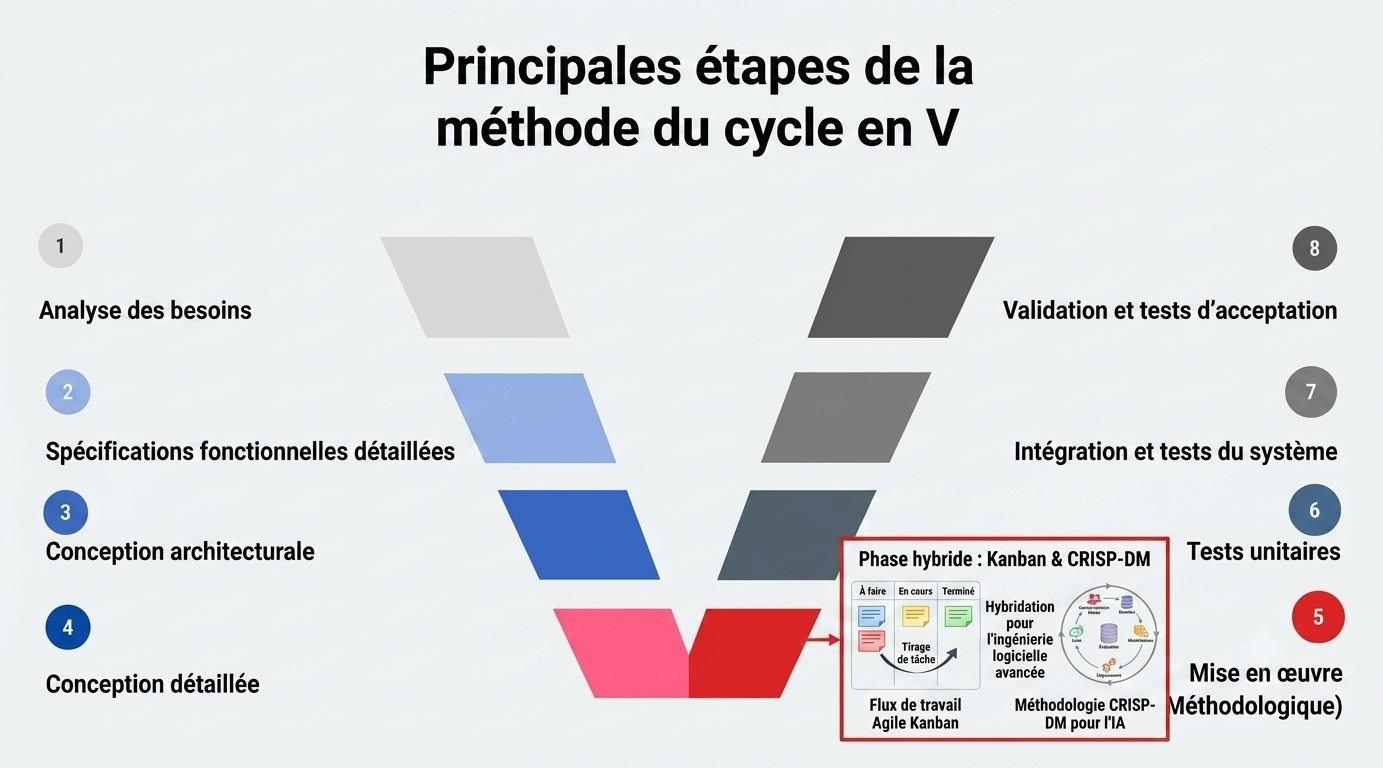
\includegraphics[width=0.85\linewidth]{public/methaoly}
	\caption{Hybridation méthodologique : Kanban et CRISP-DM imbriqués dans le Cycle en V}
	\label{fig:hybridation_v}
\end{figure}

L’hybridation n’est pas un empilement arbitraire : elle repose sur une analyse précise des forces et limites de chaque méthode (tableau~\ref{tab:comparaison_methodologies}). Le modèle en V fournit le squelette — il fixe les jalons majeurs et assure la traçabilité ascendante/descendante. À l’intérieur de ce squelette, CRISP-DM apporte l’itération nécessaire à la fouille de données, tandis que Kanban apporte la fluidité pour le développement logiciel.
Le tableau~\ref{tab:methodologies_composantes} détaille l’affectation de chaque composant ou phase à la méthode principale, tout en précisant comment l’hybridation est mise en œuvre. 

\begin{table}[!htbp]
	\centering
	\small
	\renewcommand{\arraystretch}{1.5}
	\begin{tabularx}{\textwidth}{|p{6.5cm}|X|}
		\hline
		\rowcolor[HTML]{2C3E50}
		\textcolor{white}{\textbf{Phase / Activité}} & \textcolor{white}{\textbf{Méthodologie appliquée}} \\ \hline
		\rowcolor[HTML]{EFEFEF}
		Analyse des besoins (chapitre II) & Cycle en V (cadre) \\ \hline
		Conception architecturale (chapitre III) & Cycle en V \\ \hline
		\rowcolor[HTML]{EFEFEF}
		Conception détaillée IA & CRISP-DM (itératif, intégré dans la phase de conception du V) \\ \hline
		Développement Backend (Spring Boot) & Kanban \\ \hline
		\rowcolor[HTML]{EFEFEF}
		Développement Mobile (Flutter) & Kanban \\ \hline
		Développement Interface Web (React) & Kanban \\ \hline
		\rowcolor[HTML]{EFEFEF}
		Système IoT et firmware (Arduino / Raspberry Pi) & Cycle en V  \\ \hline
		Intégration globale & Cycle en V \\ \hline
		\rowcolor[HTML]{EFEFEF}
		Validation et tests (chapitre V) & Cycle en V \\ \hline
	\end{tabularx}
	\caption{Application des méthodologies aux différentes composantes du projet}
	\label{tab:methodologies_composantes}
\end{table}

	
	\section*{Conclusion}
\addcontentsline{toc}{section}{Conclusion}

Ce premier chapitre a posé les bases du projet \textit{HydroNova} en présentant son contexte institutionnel, son environnement technologique et la méthodologie de gestion retenue. L’analyse des solutions agricoles intelligentes existantes a révélé plusieurs limitations récurrentes, notamment une forte dépendance à la connectivité Internet et aux infrastructures Cloud, ce qui restreint leur déploiement dans les zones rurales peu desservies et expose les exploitants à des risques de latence ou de panne réseau.

Ces constats justifient la conception d’une architecture originale, résiliente et capable de fonctionner en mode hors ligne, où l’intelligence est répartie entre la périphérie (Edge AI sur Raspberry Pi) et le Cloud, et où les décisions critiques sont prises localement.

Par ailleurs, l’adoption d’une approche méthodologique hybride, combinant le Cycle en V pour la rigueur et la traçabilité, Kanban pour la fluidité du développement logiciel, et CRISP‑DM pour l’itération propre à l’intelligence artificielle. Cette hybridation offre un cadre de développement à la fois structuré, flexible et adapté aux spécificités d’un projet intégrant des composantes matérielles, logicielles et IA.

Les fondements du projet étant désormais établis, le chapitre suivant entre dans la phase d’étude approfondie. Il sera consacré à un état de l’art des architectures et méthodes intelligentes appliquées au domaine agricole. Nous y examinerons les techniques d’intelligence artificielle pour la détection de maladies végétales (CNN, Vision-Language Models, apprentissage par ensemble). Cette analyse permettra de positionner les choix technologiques d’\textit{HydroNova} par rapport aux travaux antérieurs et de justifier les orientations retenues pour la suite du projet.

\include{Chapitre2}

\chapter{ANALYSE ET SPÉCIFICATION DES BESOINS}

\section*{Introduction}
\addcontentsline{toc}{section}{Introduction}

La réussite technique du \textit{HydroNova} repose sur une définition précise des attentes des utilisateurs et des exigences opérationnelles des machines. Ce chapitre détaille l'analyse des besoins en segmentant le système en quatre piliers technologiques : l'application mobile pour l'exploitant, l'interface web pour l'administration, l'infrastructure IoT pour le contrôle local, et l'intelligence artificielle pour le diagnostic sanitaire. Cette approche permet de garantir que chaque composant répond aux standards de performance et de fiabilité requis.

%================================================================
\section{Identification des Acteurs}
%================================================================

La conception d’un écosystème IoT intelligent et décentralisé nécessite une identification claire des différentes entités interagissant avec le système. Les acteurs représentent aussi bien les utilisateurs humains que les composants logiciels et matériels capables d’échanger des données ou d’exécuter des traitements autonomes.

Dans le cadre de ce projet, les acteurs sont répartis en deux catégories principales : les acteurs humains et les acteurs systémiques.


\subsection{Acteurs}

\begin{itemize}
	\item \textbf{L'Agriculteur :} Acteur principal du système et utilisateur final de l’application mobile. Il supervise les paramètres environnementaux de la serre, contrôle les équipements connectés, suit les cycles de production et exploite les outils d’assistance intelligente afin d’optimiser la production hydroponique.
	
	\item \textbf{Visiteur :} Utilisateur disposant d’un accès restreint à certaines fonctionnalités publiques de la plateforme. Il peut interagir avec le chatbot intelligent, consulter les actualités agricole .
	
	\item \textbf{L'Administrateur :} Responsable de la gestion globale de la plateforme via l’interface web d’administration. Il supervise les utilisateurs, les serres déployées, les configurations système, les droits d’accès ainsi que les opérations de maintenance et de supervision centralisée.
	
	\item \textbf{Agent Technique :} Technicien chargé des interventions techniques sur les équipements déployés. Il assure les opérations de maintenance corrective et préventive .
\end{itemize}
    %================================================================
\section{Spécification des Besoins}
%================================================================

Après l’identification des acteurs, cette section formalise les besoins fonctionnels et non fonctionnels du système. L’analyse est structurée autour des quatre piliers technologiques de la plateforme : le sous-système mobile destiné à l’exploitant, le sous-système web dédié à l’administration, le sous-système IoT assurant le contrôle local, et le sous-système d’intelligence artificielle responsable du diagnostic sanitaire.

\subsection{Sous-système Mobile}
Cette section présente les besoins fonctionnels et non fonctionnels de l’application mobile du système.
Elle décrit les principales fonctionnalités offertes aux différents types d’utilisateurs ainsi que les contraintes garantissant la qualité du service.
\subsubsection{Besoins Fonctionnels}

\begingroup
\footnotesize % Taille de police légèrement réduite pour gagner de l'espace
\setlength{\tabcolsep}{4pt} % Réduction des marges intérieures des colonnes (défaut : 6pt)
\renewcommand{\arraystretch}{1.2} % Espacement vertical plus compact et adapté au texte multiligne

\begin{longtable}{|p{0.24\textwidth}|>{\raggedright\arraybackslash}p{0.54\textwidth}|>{\raggedright\arraybackslash}p{0.16\textwidth}|}
	\hline
	\rowcolor[HTML]{2C3E50}
	\textcolor{white}{\textbf{Besoin}} &
	\textcolor{white}{\textbf{Description}} &
	\textcolor{white}{\textbf{Acteur Concerné}} \\ \hline
	\endfirsthead
	
	\hline
	\rowcolor[HTML]{2C3E50}
	\textcolor{white}{\textbf{Besoin}} &
	\textcolor{white}{\textbf{Description}} &
	\textcolor{white}{\textbf{Acteur Concerné}} \\ \hline
	\endhead
	
	\textbf{Authentification et gestion de compte} &
	Le système doit permettre aux utilisateurs de créer un compte et de s’authentifier de manière sécurisée avec gestion des accès. &
	Agriculteur, Visiteur \\ \hline
	
	\textbf{Supervision de la serre} &
	Le système doit permettre la consultation en temps réel des données environnementales de la serre. &
	Agriculteur \\ \hline
	
	\textbf{Contrôle des équipements de la serre} &
	Le système doit permettre le contrôle manuel des équipements tels que l’irrigation, l’éclairage et la ventilation ... &
	Agriculteur \\ \hline
	
	\textbf{Analyse et historique des cultures} &
	Le système doit permettre la consultation des statistiques et de l’historique des cycles de production afin de suivre l’évolution des cultures. &
	Agriculteur \\ \hline
	
	\textbf{Assistance intelligente multilingue (Chatbot)} &
	Le système doit intégrer un chatbot intelligent capable d’assister les utilisateurs en plusieurs langues et de répondre aux questions liées à l’hydroponie et à la plateforme. &
	Agriculteur, Visiteur \\ \hline
	
	\textbf{Notifications et alertes de la serre} &
	Le système doit envoyer à l’agriculteur des notifications liées aux anomalies détectées, aux alertes critiques issues des capteurs . &
	Agriculteur \\ \hline
	
	\textbf{Notifications de contenu et actualités} &
	Le système doit envoyer aux visiteurs des notifications concernant les nouvelles publications, les actualités agricoles et les mises à jour de la plateforme. &
	Visiteur \\ \hline
	
	\textbf{Abonnement aux mises à jour} &
	Le système doit permettre aux visiteurs de s’abonner afin de recevoir des notifications personnalisées liées aux contenus agricoles, au chatbot et aux nouvelles fonctionnalités de la plateforme. &
	Visiteur \\ \hline
	
	\caption{Besoins fonctionnels de l’application mobile}
	\label{tab:bf-mobile}
\end{longtable}
\endgroup
\subsubsection{Besoins Non Fonctionnels}


\begingroup
\footnotesize % Taille de police légèrement réduite pour gagner de l'espace
\setlength{\tabcolsep}{4pt} % Réduction des marges intérieures des colonnes
\renewcommand{\arraystretch}{1.2} % Espacement vertical plus compact et adapté au texte multiligne

\begin{longtable}{|>{\raggedright\arraybackslash}p{4cm}|>{\raggedright\arraybackslash}p{10cm}|}
	\hline
	\rowcolor[HTML]{2C3E50}
	\textcolor{white}{\textbf{Critère}} & \textcolor{white}{\textbf{Exigence Technique}}
	\\ \hline
	\endfirsthead
	
	\hline
	\rowcolor[HTML]{2C3E50}
	\textcolor{white}{\textbf{Critère}} & \textcolor{white}{\textbf{Exigence Technique}}
	\\ \hline
	\endhead
	
	\textbf{Performance} &
	L’application mobile doit garantir une faible latence dans l’affichage des données critiques afin d’assurer une expérience utilisateur fluide et réactive.
	\\ \hline
	
	\textbf{Réactivité} &
	L’interface doit rester fluide même en cas de forte charge, avec une gestion optimisée des mises à jour via un mécanismes équivalents.
	\\ \hline
	
	\textbf{Disponibilité} &
	Le système doit assurer une disponibilité continue des fonctionnalités essentielles. 
	\\ \hline
	
	\textbf{Sécurité} &
	L’accès à l’application doit être sécurisé par authentification , avec chiffrement des échanges entre le client mobile et le backend.
	\\ \hline
	
	\textbf{Ergonomie} &
	L’interface utilisateur doit être intuitive, responsive et adaptée à une utilisation sur le terrain, même dans des conditions d’usage difficiles.
	\\ \hline
	
	\textbf{Compatibilité} &
	L’application doit être compatible avec les systèmes Android et iOS, garantissant une expérience utilisateur homogène sur différentes plateformes.
	\\ \hline
	
	\textbf{Scalabilité} &
	L’architecture doit permettre la montée en charge du nombre d’utilisateurs et de serres connectées sans dégradation notable des performances.
	\\ \hline
	
	\textbf{Robustesse} &
	Le système doit rester fonctionnel en cas de coupures réseau intermittentes, avec synchronisation automatique lors de la reconnexion.
	\\ \hline
	
	\caption{Besoins non fonctionnels de l’application mobile}
	\label{tab:nf-mobile}
\end{longtable}
\endgroup
%================================================================

%----------------------------------------------------------------
\subsection{Sous-système Web}

Cette section présente les besoins fonctionnels et non fonctionnels du sous-système web de la plateforme.  
Elle décrit les fonctionnalités dédiées à la supervision, à la gestion du système ainsi qu’à l’administration des équipements et des utilisateurs.
\subsubsection{Besoins Fonctionnels}

\begingroup
\footnotesize % Taille de police légèrement réduite pour gagner de l'espace
\setlength{\tabcolsep}{4pt} % Réduction des marges intérieures des colonnes
\renewcommand{\arraystretch}{1.5} % Espacement vertical choisi

{\small
	\renewcommand{\arraystretch}{1.5}
	\begin{longtable}{|>{\raggedright\arraybackslash}p{4cm}|>{\raggedright\arraybackslash}p{9cm}|>{\raggedright\arraybackslash}p{3cm}|}
		
		\hline
		\rowcolor[HTML]{2C3E50}
		\textcolor{white}{\textbf{Besoin}} &
		\textcolor{white}{\textbf{Description}} &
		\textcolor{white}{\textbf{Acteur Concerné}}
		\\ \hline
		\endfirsthead
		
		\hline
		\rowcolor[HTML]{2C3E50}
		\textcolor{white}{\textbf{Besoin}} &
		\textcolor{white}{\textbf{Description}} &
		\textcolor{white}{\textbf{Acteur Concerné}}
		\\ \hline
		\endhead
		
		\rowcolor[HTML]{EFEFEF}
		\textbf{Gestion des comptes utilisateurs} &
		Le système doit permettre la création, la modification, la suspension et la suppression des comptes utilisateurs. &
		Administrateur
		\\ \hline
		
		\textbf{Gestion des rôles et permissions (RBAC)} &
		Le système doit permettre la définition et la gestion des rôles ainsi que des droits d’accès selon les profils utilisateurs. &
		Administrateur
		\\ \hline
		
		\rowcolor[HTML]{EFEFEF}
		\textbf{Supervision globale des serres} &
		Le système doit fournir une vue centralisée de l’état des serres et des équipements connectés. &
		Administrateur, Agent Technique
		\\ \hline
		
		\textbf{Gestion des équipements IoT} &
		Le système doit permettre l’enregistrement, la configuration et la supervision des capteurs et actionneurs installés dans les serres. &
		Agent Technique
		\\ \hline
		
		\rowcolor[HTML]{EFEFEF}
		\textbf{Analyse et statistiques globales} &
		Le système doit fournir des tableaux de bord analytiques permettant le suivi des performances de la plateforme et des serres. &
		Administrateur
		\\ \hline
		
		\textbf{Gestion des contenus et actualités} &
		Le système doit permettre la création, la modification et la publication d’articles destinés aux utilisateurs de la plateforme. &
		Administrateur
		\\ \hline
		
		\rowcolor[HTML]{EFEFEF}
		
		
		\textbf{Gestion des interventions techniques} &
		Le système doit permettre la création, la consultation et le suivi des tickets d’intervention liés aux équipements des serres. &
		Agent Technique
		\\ \hline
		
		\rowcolor[HTML]{EFEFEF}
		
		
		\textbf{Déploiement des mises à jour} &
		Le système doit permettre la mise à jour à distance des équipements, capteurs, actionneurs et modules logiciels. &
		Agent Technique
		\\ \hline
		
		\caption{Besoins fonctionnels de l’application web (Administrateur et Agent Technique)}
		\label{tab:bf-web-combined}
		
	\end{longtable}
}
\endgroup
% ==========================================================
\subsubsection{Besoins Non Fonctionnels}

\renewcommand{\arraystretch}{1.5}

{\small
	\renewcommand{\arraystretch}{1.5}
	\begin{longtable}{|p{4cm}|p{9cm}|}
		
		\hline
		\rowcolor[HTML]{2C3E50}
		\textcolor{white}{\textbf{Critère}} &
		\textcolor{white}{\textbf{Exigence}}
		\\ \hline
		\endfirsthead
		
		\hline
		\rowcolor[HTML]{2C3E50}
		\textcolor{white}{\textbf{Critère}} &
		\textcolor{white}{\textbf{Exigence}}
		\\ \hline
		\endhead
		
		\rowcolor[HTML]{EFEFEF}
		\textbf{Scalabilité} &
		Le système doit supporter l’augmentation du nombre de serres et d’utilisateurs sans dégradation des performances.
		\\ \hline
		
		\textbf{Fiabilité} &
		Le système doit garantir l’intégrité et la cohérence des données enregistrées.
		\\ \hline
		
		\rowcolor[HTML]{EFEFEF}
		\textbf{Sécurité renforcée} &
		Les opérations critiques doivent être protégées par des mécanismes de sécurité avancés.
		\\ \hline
		
		\textbf{Performance} &
		L’interface web doit offrir des temps de chargement rapides afin d’améliorer la productivité des utilisateurs.
		\\ \hline
		
		\rowcolor[HTML]{EFEFEF}
		\textbf{Traçabilité} &
		Toutes les opérations importantes doivent être journalisées afin de faciliter les audits et la maintenance.
		\\ \hline
		
		\caption{Besoins non fonctionnels de l’interface web}
		\label{tab:bnf-web}
		
	\end{longtable}
}
%----------------------------------------------------------------
\subsection{Sous-système IoT}

Le système embarqué constitue le cœur opérationnel de la serre intelligente. Il assure le contrôle local des équipements ainsi que la collecte des données en périphérie (Edge Computing), garantissant ainsi l’autonomie du système même en cas de perte de connectivité.

% ==========================================================
\subsubsection{Besoins Fonctionnels}

{\small
	\renewcommand{\arraystretch}{1.5}
	\begin{longtable}{|p{4cm}|p{9cm}|}

		\hline
		\rowcolor[HTML]{2C3E50}
		\textcolor{white}{\textbf{Besoin}} &
		\textcolor{white}{\textbf{Description}}
		\\ \hline
		\endfirsthead

		\hline
		\rowcolor[HTML]{2C3E50}
		\textcolor{white}{\textbf{Besoin}} &
		\textcolor{white}{\textbf{Description}}
		\\ \hline
		\endhead

		\rowcolor[HTML]{EFEFEF}
		\textbf{Collecte des données environnementales} &
		Le système doit assurer l’acquisition continue et périodique des données provenant des capteurs environnementaux (température, humidité, CO2 ...). 
		\\ \hline
		
		\textbf{Communication IoT avec le backend} &
		Le système doit transmettre les données télémétriques vers le backend et recevoir les commandes de contrôle des équipements de la serre. 
		\\ \hline
		
		\rowcolor[HTML]{EFEFEF}
		\textbf{Contrôle autonome de la serre} &
		Le système doit garantir le fonctionnement des équipements critiques (irrigation, ventilation, détection de maladie , ... ) de manière autonome en cas de perte de connexion réseau. 
		\\ \hline
		
		\textbf{Synchronisation des données locales} &
		Le système doit synchroniser automatiquement les données stockées localement avec le backend dès le rétablissement de la connexion réseau. 
		\\ \hline
		
		\caption{Besoins fonctionnels du système embarqué}
		\label{tab:bf-embedded}
		
	\end{longtable}
}
% ==========================================================
\subsubsection{Besoins Non Fonctionnels}

\renewcommand{\arraystretch}{1.5}

{\small
	\renewcommand{\arraystretch}{1.5}
	\begin{longtable}{|p{4cm}|p{9cm}|}
		
		\hline
		\rowcolor[HTML]{2C3E50}
		\textcolor{white}{\textbf{Critère}} &
		\textcolor{white}{\textbf{Exigence}}
		\\ \hline
		\endfirsthead
		
		\hline
		\rowcolor[HTML]{2C3E50}
		\textcolor{white}{\textbf{Critère}} &
		\textcolor{white}{\textbf{Exigence}}
		\\ \hline
		\endhead
		
		\rowcolor[HTML]{EFEFEF}
		\textbf{Disponibilité} &
		Le système embarqué doit garantir un fonctionnement continu afin d’assurer la survie des cultures et la stabilité de la serre.
		\\ \hline
		
		\textbf{Optimisation des ressources} &
		Le système doit limiter la consommation mémoire et CPU afin de rester compatible avec les capacités matérielles du matériel embarqué.
		\\ \hline
		
		\caption{Besoins non fonctionnels du système embarqué}
		\label{tab:bnf-embedded}
		
	\end{longtable}
}

%----------------------------------------------------------------
\subsection{Sous-système d'Intelligence Artificielle}

Le sous-système d’intelligence artificielle constitue le module central chargé de l’analyse automatique des données visuelles et de la détection des anomalies phytosanitaires.

% ==========================================================
\subsubsection{Besoins Fonctionnels}

{\small
	\renewcommand{\arraystretch}{1.5}
	\begin{longtable}{|p{4cm}|p{9cm}|}
		
		\hline
		\rowcolor[HTML]{2C3E50}
		\textcolor{white}{\textbf{Besoin}} &
		\textcolor{white}{\textbf{Description}}
		\\ \hline
		\endfirsthead
		
		\hline
		\rowcolor[HTML]{2C3E50}
		\textcolor{white}{\textbf{Besoin}} &
		\textcolor{white}{\textbf{Description}}
		\\ \hline
		\endhead
		
		\rowcolor[HTML]{EFEFEF}
		\textbf{Analyse intelligente des images (Edge AI)} &
		Le module d’intelligence artificielle doit analyser localement les images capturées afin de détecter les maladies, carences et anomalies affectant les cultures. 
		\\ \hline
		

		
		
		\caption{Besoins fonctionnels du module IA}
		\label{tab:bf-ia}
		
	\end{longtable}
}
% ==========================================================
\subsubsection{Besoins Non Fonctionnels}

\renewcommand{\arraystretch}{1.5}

{\small
	\renewcommand{\arraystretch}{1.5}
	\begin{longtable}{|p{4cm}|p{9cm}|}
		
		\hline
		\rowcolor[HTML]{2C3E50}
		\textcolor{white}{\textbf{Critère}} &
		\textcolor{white}{\textbf{Exigence}}
		\\ \hline
		\endfirsthead
		
		\hline
		\rowcolor[HTML]{2C3E50}
		\textcolor{white}{\textbf{Critère}} &
		\textcolor{white}{\textbf{Exigence}}
		\\ \hline
        
		\endhead
		\rowcolor[HTML]{EFEFEF}
		\textbf{Certitude des prédictions} &
		Le modèle d'IA doit bien connaître les caractéristiques des maladies afin de garantir un niveau de certitude élevé lors des détections.
		\\ \hline

		\caption{Besoins non fonctionnels du module IA}
		\label{tab:bnf-ia}
		
	\end{longtable}
}
Ainsi, afin de représenter de manière claire, structurée et normalisée les besoins fonctionnels et non fonctionnels du système, il est nécessaire d’adopter un langage de modélisation adapté à la conception et à la formalisation de l’architecture logicielle.

%================================================================
\sectiontitle{Langage de modélisation}
%================================================================

Dans le cadre de ce projet, la définition des besoins et la conception du système nécessitent une représentation standardisée et compréhensible par l’ensemble des parties prenantes. Pour cela, nous avons retenu le langage UML (Unified Modeling Language), qui constitue aujourd’hui un standard incontournable dans le domaine du génie logiciel.

L’UML est un langage graphique basé sur un ensemble de diagrammes permettant de représenter visuellement la structure statique et le comportement dynamique d’un système. Il est largement utilisé dans les projets orientés objet, mais peut également être appliqué à d’autres domaines nécessitant une modélisation claire et structurée.

\subsectiontitle{Pourquoi utiliser UML ?}

L’UML est un langage formel et standardisé qui facilite la modélisation des systèmes complexes. Son principal avantage réside dans son indépendance vis-à-vis des langages de programmation, ce qui en fait un outil universel de conception.

Il permet avant tout d’assurer une meilleure communication entre les différents acteurs d’un projet (développeurs, concepteurs, décideurs) grâce à une représentation visuelle commune et normalisée. Cette formalisation contribue à réduire les ambiguïtés, à améliorer la compréhension des besoins et à garantir une meilleure cohérence globale de la conception.

Dans ce chapitre, UML est utilisé comme support principal pour la modélisation des cas d’utilisation et la spécification des besoins du système.



\subsectiontitle{Dynamique Globale des Cas d'Utilisation}

Le diagramme des cas d'utilisation permet de définir les frontières fonctionnelles du système en identifiant les différents acteurs ainsi que les interactions qu’ils peuvent effectuer avec la plateforme. Il met en évidence les flux opérationnels autorisés pour chaque acteur et précise les responsabilités associées au système.

La représentation globale de ces interactions est illustrée par le diagramme suivant :



Comme le montre la figure~\ref{fig:usekbir}, le système est structuré autour de plusieurs acteurs et cas d’utilisation, permettant de visualiser clairement les fonctionnalités offertes ainsi que les échanges entre les différentes entités.
\begin{figure}[!h]
	\centering
	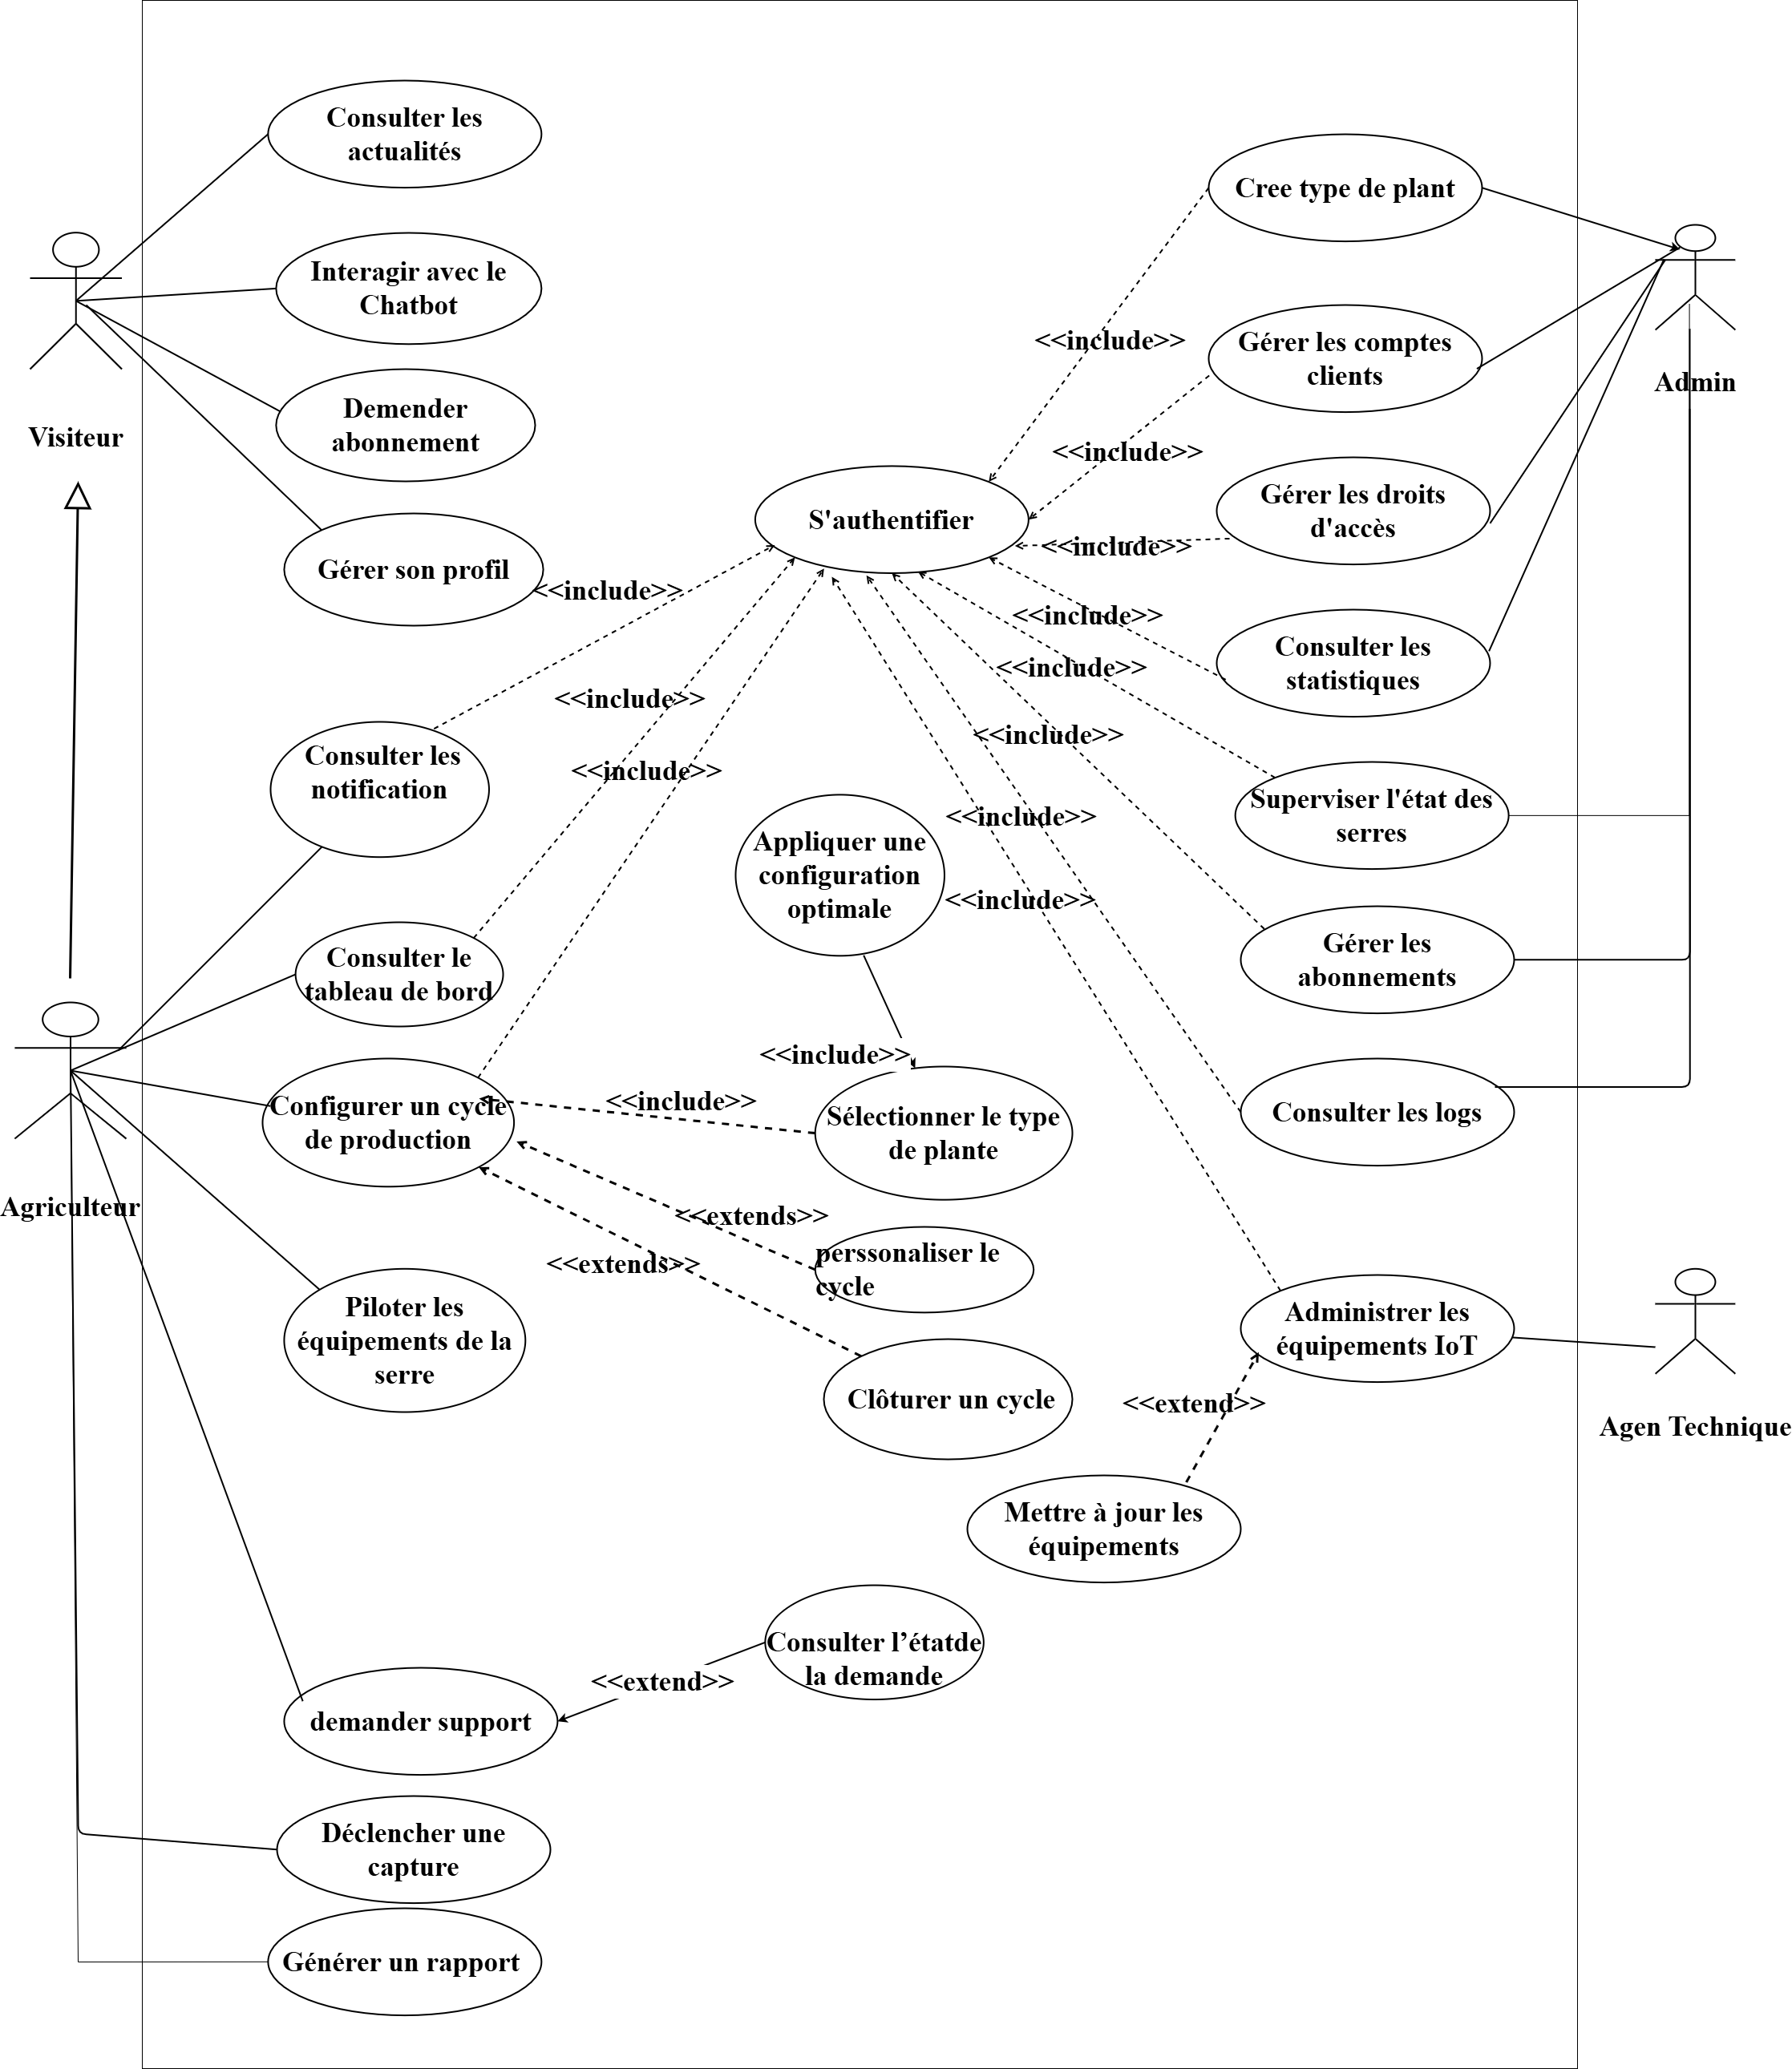
\includegraphics[width=1\linewidth]{public/casecase.drawio.png}
	\caption{Diagramme des cas d’utilisation du système}
	\label{fig:usekbir}
\end{figure}
\subsectiontitle{Diagramme de classe}
Le diagramme de classe métier présenté par la figure~\ref{fig:classanlse} décrit les entités clés intervenant dans le fonctionnement du système ainsi que leurs associations.
\begin{landscape} % active le mode paysage
\begin{figure}[tbph!]
	\centering
	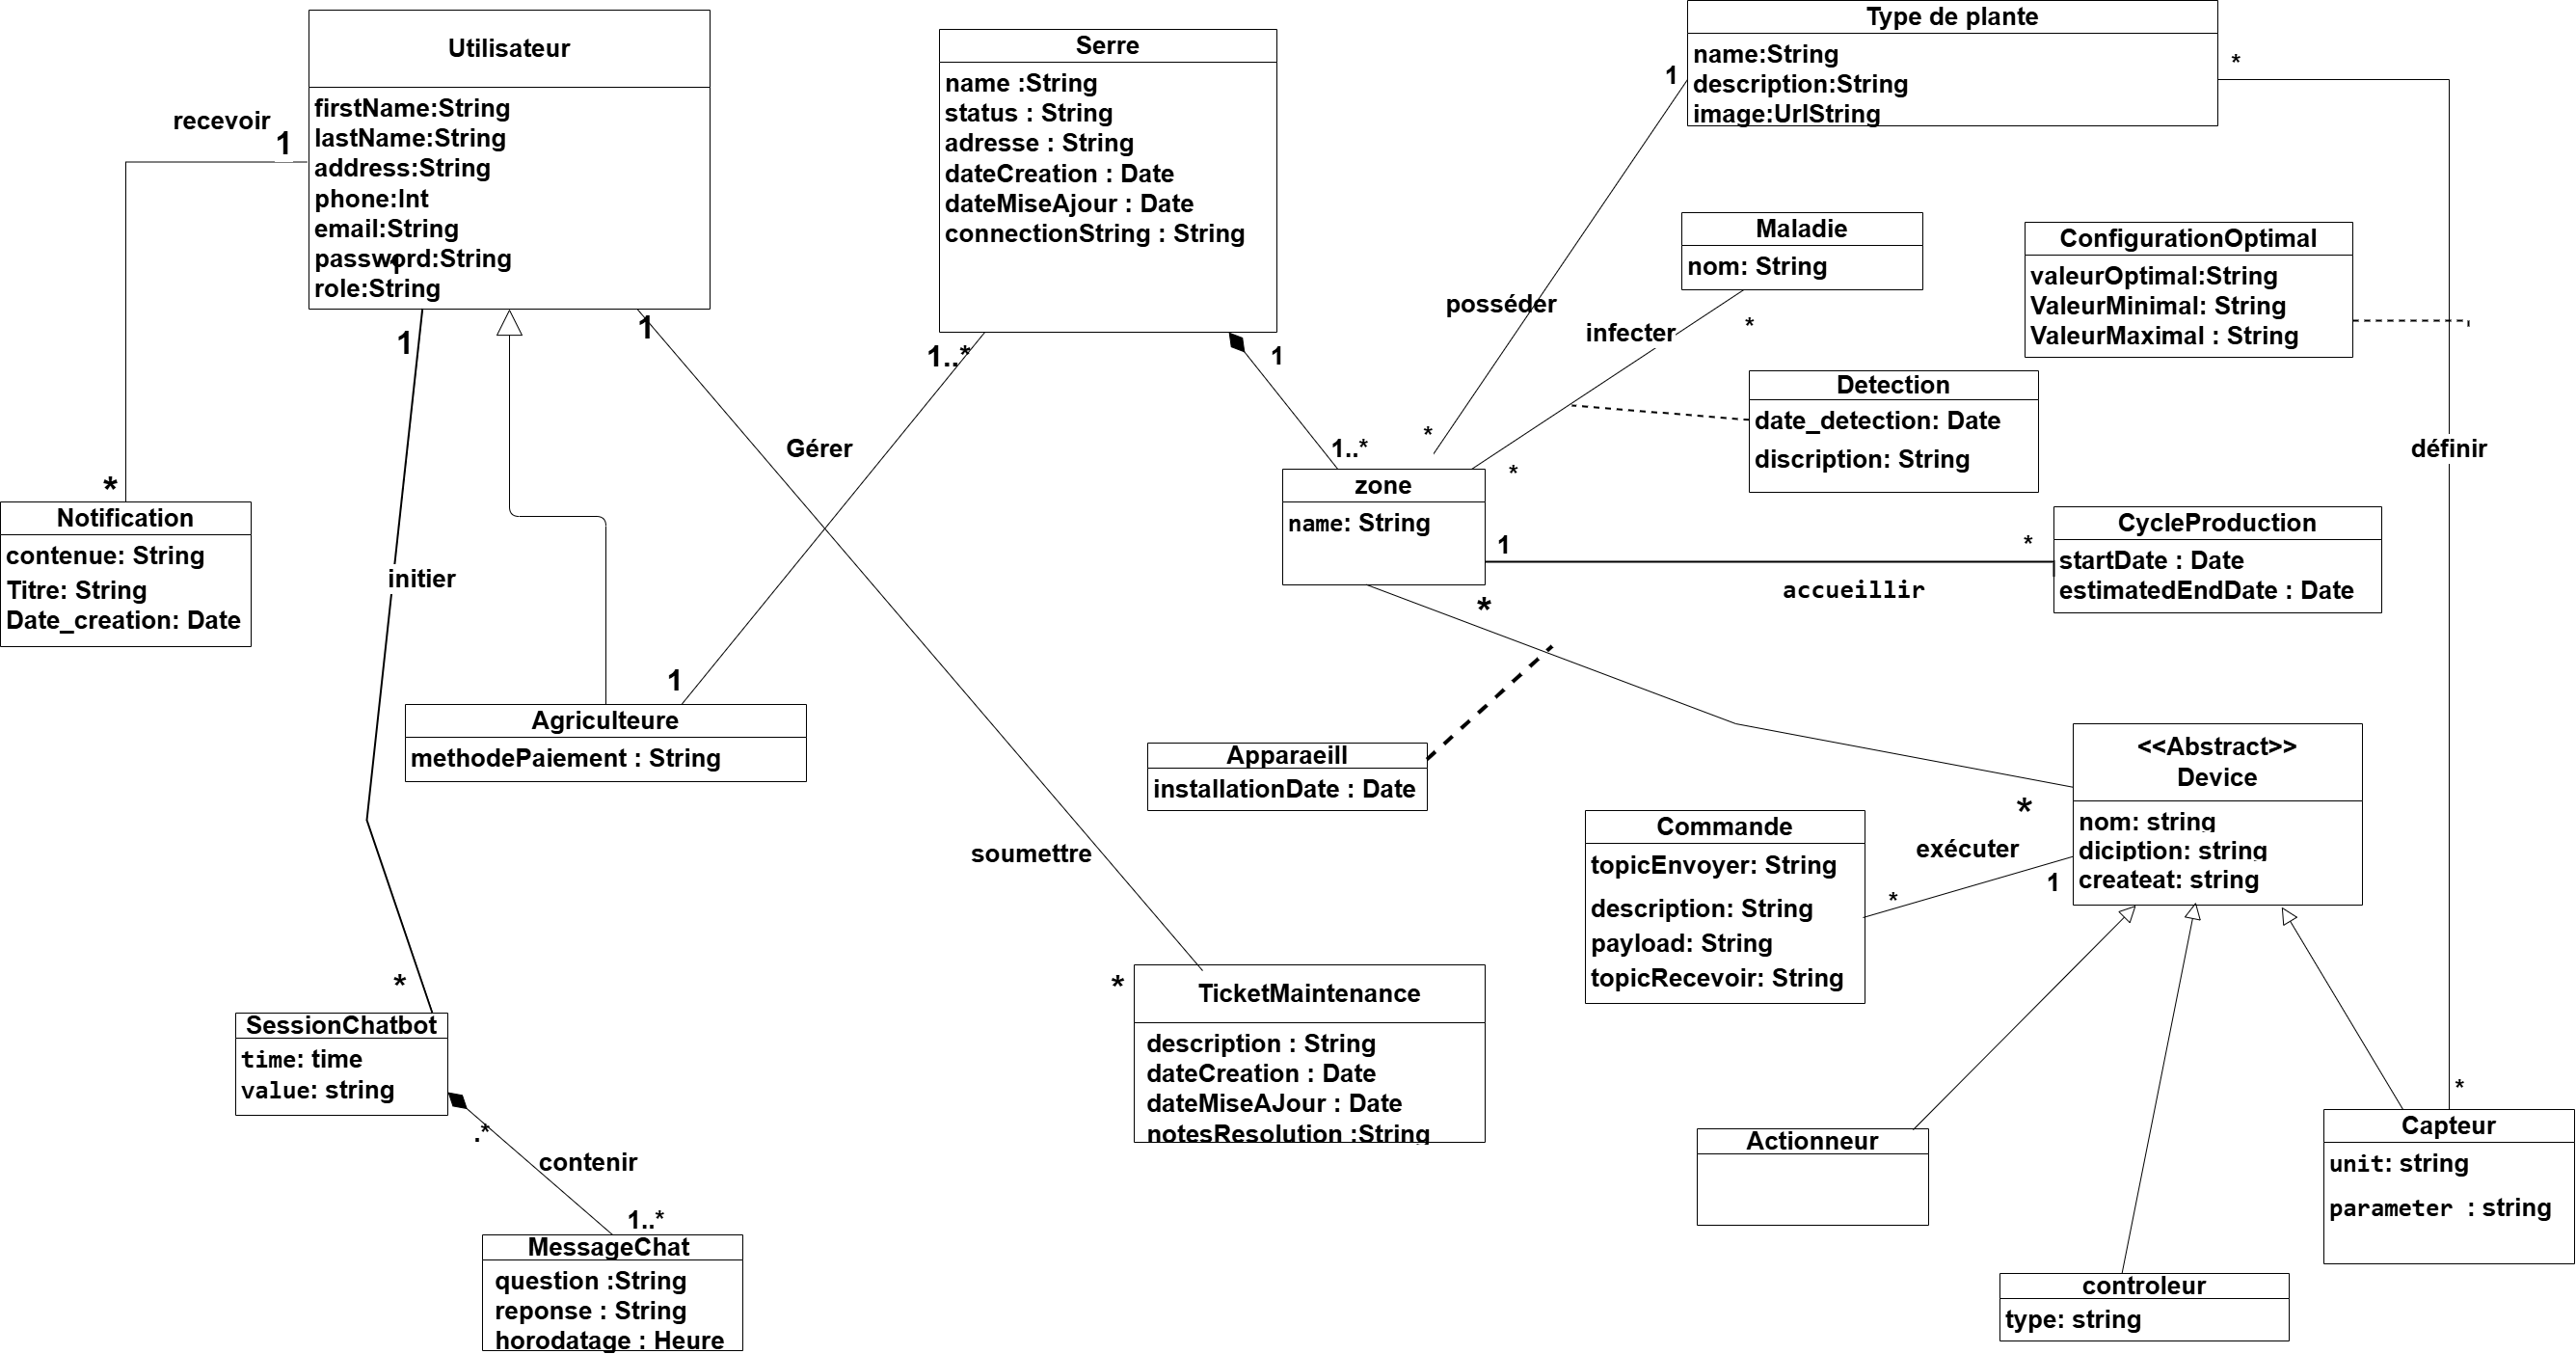
\includegraphics[width=1\linewidth]{public/classy.drawio}
	\caption{Diagramme de classes Analyse}
	\label{fig:classanlse}
\end{figure}
\end{landscape}

\section*{Conclusion}
\addcontentsline{toc}{section}{Conclusion}

Ce chapitre a permis de formaliser l’analyse et la spécification des besoins du système \textit{HydroNova}. Après avoir identifié les différents acteurs intervenant dans la plateforme, nous avons recensé de manière structurée les besoins fonctionnels et non fonctionnels propres à chacun des quatre sous-systèmes : l’application mobile de l’exploitant, l’interface web d’administration, l’infrastructure IoT embarquée et le module d’intelligence artificielle.

Cette spécification a ensuite été consolidée par une modélisation UML, à travers le diagramme des cas d’utilisation et le diagramme de classes, offrant une représentation claire et normalisée des interactions et des entités du système. L’ensemble constitue une base rigoureuse garantissant la traçabilité entre les exigences exprimées et les choix techniques à venir.

Les besoins étant désormais clairement établis et formalisés, le chapitre suivant aborde la phase de conception. Il détaillera l’architecture globale de la solution ainsi que les choix de conception adoptés afin de répondre aux exigences fonctionnelles et non fonctionnelles identifiées dans ce chapitre.
% ============================================================
% CHAPITRE II — ÉTAT DE L'ART
% ============================================================
\chapter{ARCHITECTURE ET CONCEPTION}

\section*{Introduction}
\addcontentsline{toc}{section}{Introduction}

Ce chapitre présente l’architecture globale du système ainsi que les principaux choix de conception adoptés afin de répondre aux exigences fonctionnelles et non fonctionnelles du projet. Dans un contexte où le système intègre des objets connectés, des modules d’intelligence artificielle et des interfaces multi-utilisateurs, la définition d’une architecture claire et structurée constitue un enjeu essentiel pour garantir la cohérence, la maintenabilité et l’évolutivité de la solution.

Afin de maîtriser cette complexité, une approche architecturale en couches a été adoptée. Cette décomposition permet d’isoler les responsabilités de chaque composant du système, en distinguant les fonctions liées à l’acquisition des données, à la communication, au traitement centralisé et à l’interaction utilisateur. Chaque couche est conçue de manière indépendante tout en restant fortement interconnectée avec les autres, assurant ainsi une bonne interopérabilité et une meilleure robustesse globale.

Dans la suite de ce chapitre, l’architecture est analysée selon une décomposition en modules fonctionnels complémentaires. Le module IoT présente les équipements de la serre ainsi que les dispositifs embarqués assurant la collecte et le contrôle des données. Le module d’intelligence artificielle décrit les architectures mises en œuvre pour les modèles développés ainsi que les approches méthodologiques adoptées. Le module backend et communication détaille les mécanismes d’orchestration et d’échange des données entre les différents composants. Enfin, le module des interfaces utilisateur expose les environnements de supervision et d’interaction destinés aux différents profils d’utilisateurs.

Cette organisation progressive permet d’assurer une compréhension claire et structurée de l’ensemble de l’architecture du système.
\newpage
% ============================================================
\section{Architecture Globale}
\label{sec:glob}

\subsection{Modèle de référence IoT à 4 couches}
L’architecture du \textit{HydroNova} repose sur un principe fondamental de séparation des responsabilités. Inspirée des modèles de référence de l’Internet des Objets (IoT), cette architecture organise le système en plusieurs couches fonctionnelles indépendantes mais interconnectées. Une telle structuration permet d’assurer une meilleure évolutivité, une maintenance simplifiée ainsi qu’une communication fluide entre les différents composants matériels et logiciels du système.

Le choix d’une architecture IoT en quatre couches répond également aux contraintes spécifiques du contexte agricole intelligent, notamment la nécessité d’un traitement local rapide, la transmission fiable des données, la supervision centralisée et l’accès distant aux services de la plateforme.

Le modèle retenu se compose des couches suivantes :

\begin{itemize}
	
	\item \textbf{Couche 1: Objets et Composants IoT :}  
	Cette couche constitue le niveau physique du système et regroupe l’ensemble des équipements déployés dans la serre. Elle assure la collecte des données environnementales à travers les capteurs, le contrôle des équipements via les actionneurs ainsi que l’exécution locale des traitements embarqués. Elle intègre également un module d’intelligence artificielle embarquée permettant l’analyse locale des images afin de détecter les anomalies ou maladies des cultures. Cette approche réduit la dépendance au cloud, diminue la latence et garantit la continuité du fonctionnement même en cas de perte de connexion réseau.
	
	\item \textbf{Couche 2: Communication et Transport des Données :}  
	Cette couche assure la connectivité entre les dispositifs IoT, la plateforme centrale et les interfaces utilisateur. Son rôle principal consiste à garantir l’échange fiable, sécurisé et bidirectionnel des données et des commandes entre les différentes composantes du système. Elle prend en charge la transmission des données de télémétrie, des alertes intelligentes ainsi que des commandes de contrôle envoyées vers les équipements de la serre. Cette séparation de la couche réseau améliore l’interopérabilité entre les dispositifs et facilite l’intégration future de nouveaux équipements ou services.
	
	\item \textbf{Couche 3: Cloud et Backend :}  
	Cette couche représente le centre de traitement et d’orchestration du système. Elle assure la persistance des données, l’exécution de la logique métier, l’analyse des informations collectées ainsi que la gestion des utilisateurs et des droits d’accès. Elle centralise également les services intelligents de la plateforme et coordonne les interactions entre les objets connectés et les applications clientes. Cette couche permet d’exploiter les données historiques afin de générer des analyses, des alertes et des recommandations destinées à l’aide à la décision agricole.
	
	\item \textbf{Couche 4: Présentation :}  
	Cette couche correspond aux interfaces de communication entre le système et les utilisateurs finaux. Elle fournit des outils de visualisation, de supervision et de contrôle permettant de consulter l’état de la serre, suivre les données en temps réel et interagir avec les différents services disponibles. Elle comprend une application mobile destinée aux agriculteurs et aux visiteurs ainsi qu’une plateforme web dédiée aux administrateurs et aux agents techniques. Cette couche facilite le pilotage à distance et améliore l’accessibilité globale du système.
	
\end{itemize}

L’adoption de cette architecture en couches permet ainsi de garantir une meilleure modularité du système, une séparation claire des responsabilités ainsi qu’une plus grande flexibilité pour l’évolution future de la plateforme.

\begin{figure}[!htbp]
	\centering
	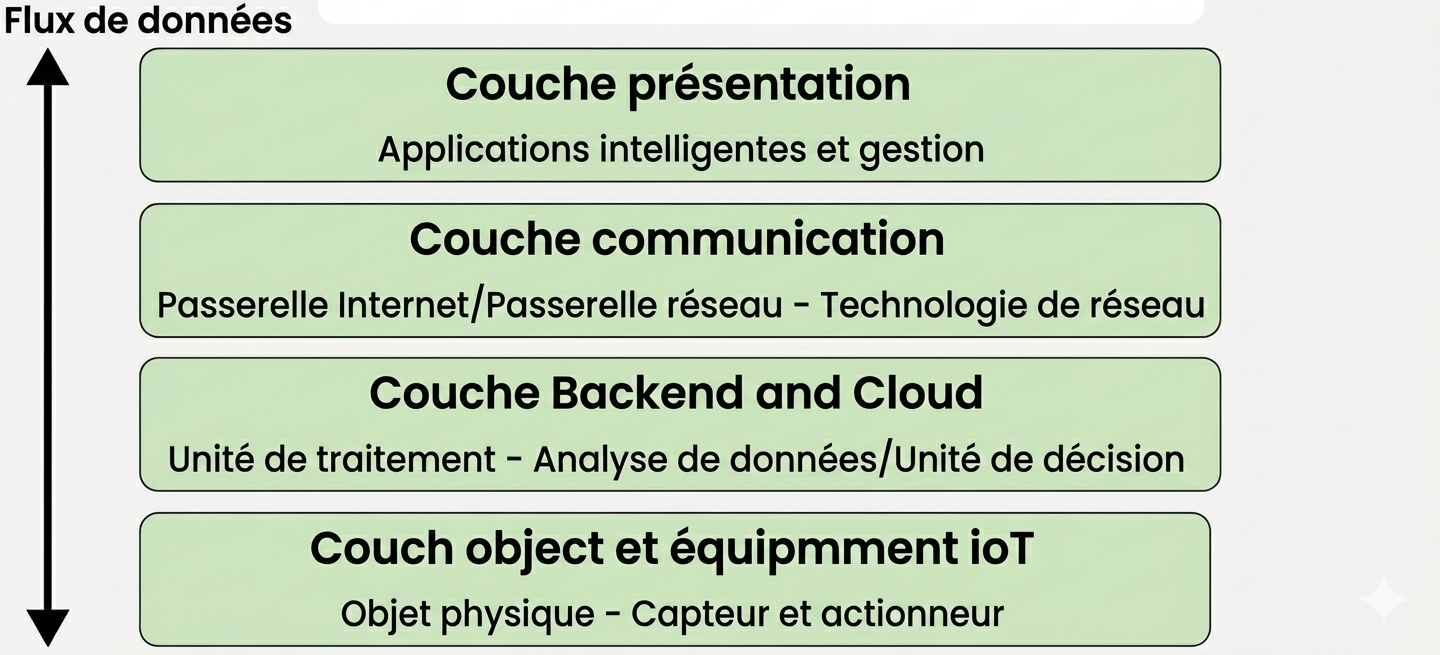
\includegraphics[width=0.7\linewidth]{public/4couche}
	\caption{Modèle IoT en 4 couches}
	\label{fig:4couche}
\end{figure}


\subsection{Flux de données global: bout en bout}
La figure \ref{fig:archi_globale} illustre cette architecture en mettant en évidence l’organisation en couches ainsi que les flux de communication entre les différents niveaux du système. Elle permet de visualiser clairement la séparation des responsabilités et le rôle de chaque composant dans le fonctionnement global de la solution.
\begin{figure}[!htbp]
	\centering
	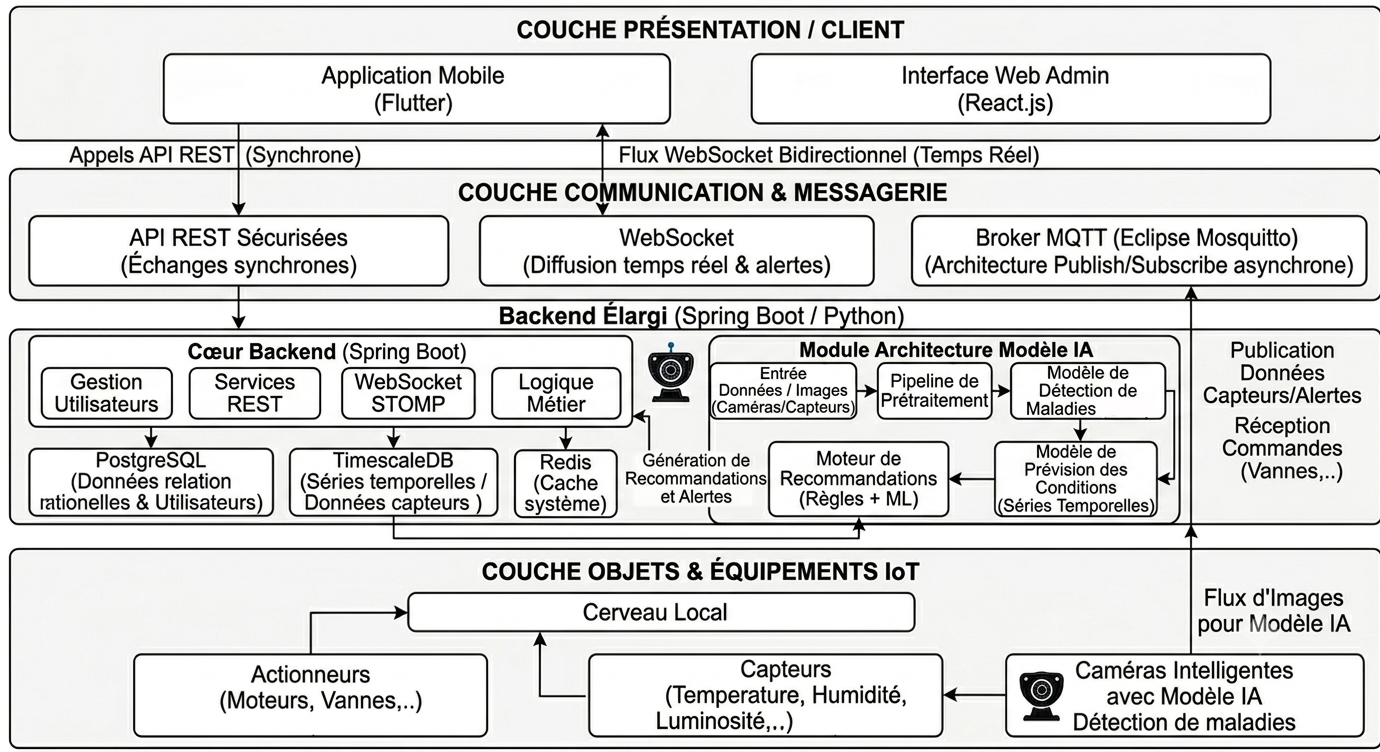
\includegraphics[width=0.95\linewidth]{public/glob.png}
	\caption{Architecture globale du système en quatre couches fonctionnelles}
	\label{fig:archi_globale}
\end{figure}


\newpage

% ============================================================
\section{Architecture Détaillée}
\label{sec:Architecture Détaillée}
% La section IA a été déplacée dans le Chapitre IV (chapitre_ia.tex)
\subsection{Module IoT et Système Embarqué}
%━━━━━━━━━━━━━━━━━━━━━━━━━━━━━━━━━━━━━━━━━━━━━━━━━━━━━━━━━━
\subsubsection{Architecture du module IoT}
L'un des principes directeurs de notre conception est l'\textbf{indépendance vis-à-vis du matériel} : l'architecture du module IoT n'est liée à aucun type de contrôleur particulier. Elle a été pensée comme un cadre générique et extensible, capable d'accueillir n'importe quelle unité de calcul embarquée (Raspberry Pi, BeagleBone, contrôleur industriel, etc.) dès lors que celle-ci respecte le contrat de communication défini par la plateforme. Pour le prototype présenté dans ce projet, le contrôleur retenu se compose d'un \textbf{Raspberry Pi 4} jouant le rôle d'unité Edge, complété par une carte \textbf{Arduino Uno} dédiée à la gestion bas niveau des entrées/sorties matérielles. Ce choix illustre une instanciation possible de l'architecture, sans en constituer une contrainte structurelle.

Cette indépendance s'étend au-delà du seul contrôleur : \textbf{capteurs et actionneurs sont eux aussi des composants extensibles}. Le principe fondateur est qu'à chaque composant physique présent dans la serre correspond une entité dans le backend. Un capteur de température installé sur l'Arduino, une pompe pilotée par un relais, un moteur pas à pas: chacun de ces éléments matériels dispose d'une représentation dans le modèle de données du serveur, portant ses caractéristiques (unité de mesure, commandes supportées, topics de communication). L'intégration d'un nouveau composant physique se résume donc à le déclarer dans ce référentiel commun, sans aucune refonte structurelle ni du micrologiciel ni du backend. C'est cette correspondance biunivoque entre le monde physique et le modèle logiciel qui garantit la compatibilité permanente entre les deux couches et qui permet à l'ensemble du système d'évoluer de façon cohérente.
\subsubsection*{Architecture matérielle de la serre}

La figure~\ref{fig:archi_iot} illustre l’architecture globale du système embarqué de la serre. Elle met en évidence l’organisation des différents composants matériels, notamment les capteurs et les actionneurs, ainsi que leur connexion à la carte Arduino. On y observe également la liaison de communication série assurant l’échange de données entre l’Arduino et le Raspberry Pi 4, qui joue le rôle de passerelle intelligente vers le système de traitement.

\begin{figure}[!htbp]
	\centering
	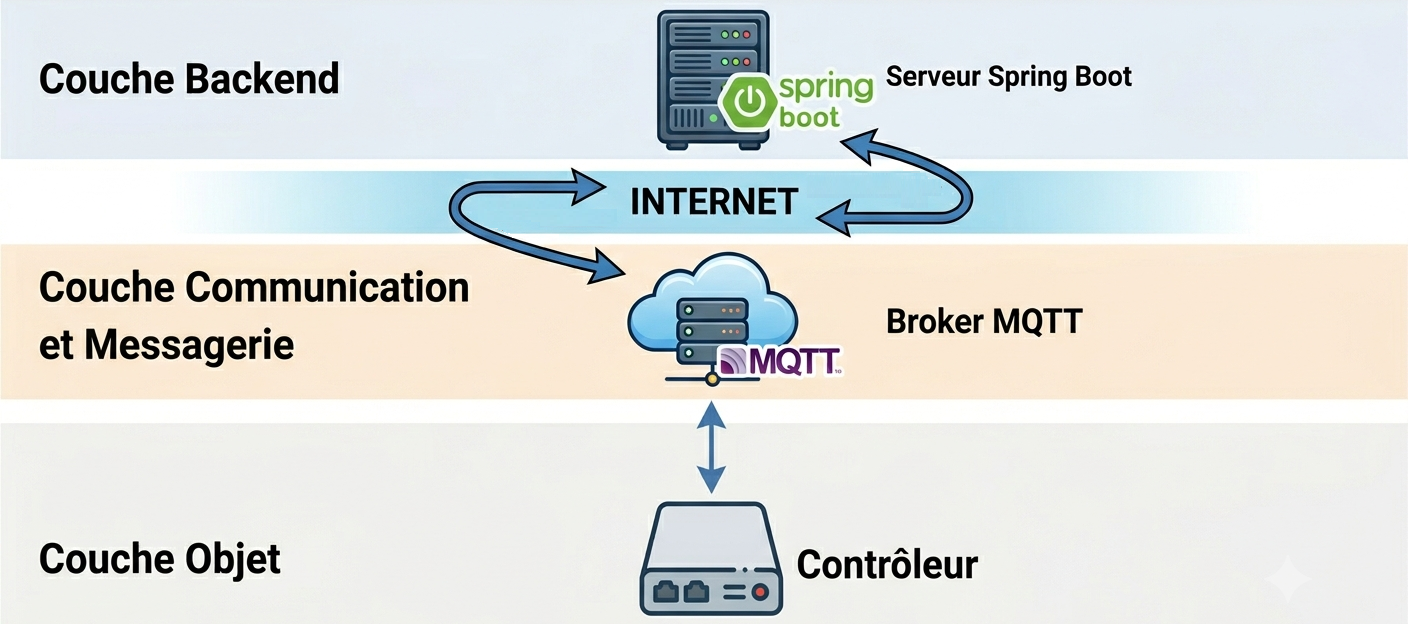
\includegraphics[width=0.8\linewidth]{public/archi_IOTF}
	\caption{Architecture globale du système IoT de la serre intelligente}
	\label{fig:archi_iot}
\end{figure}

Afin de détailler davantage l’implémentation physique du système, la figure~\ref{fig:cablage} présente le schéma de câblage des capteurs et des actionneurs connectés au contrôleur principal. Elle permet de visualiser précisément les connexions électriques et la répartition des composants au sein de la serre.

\begin{figure}[!htbp]
	\centering
	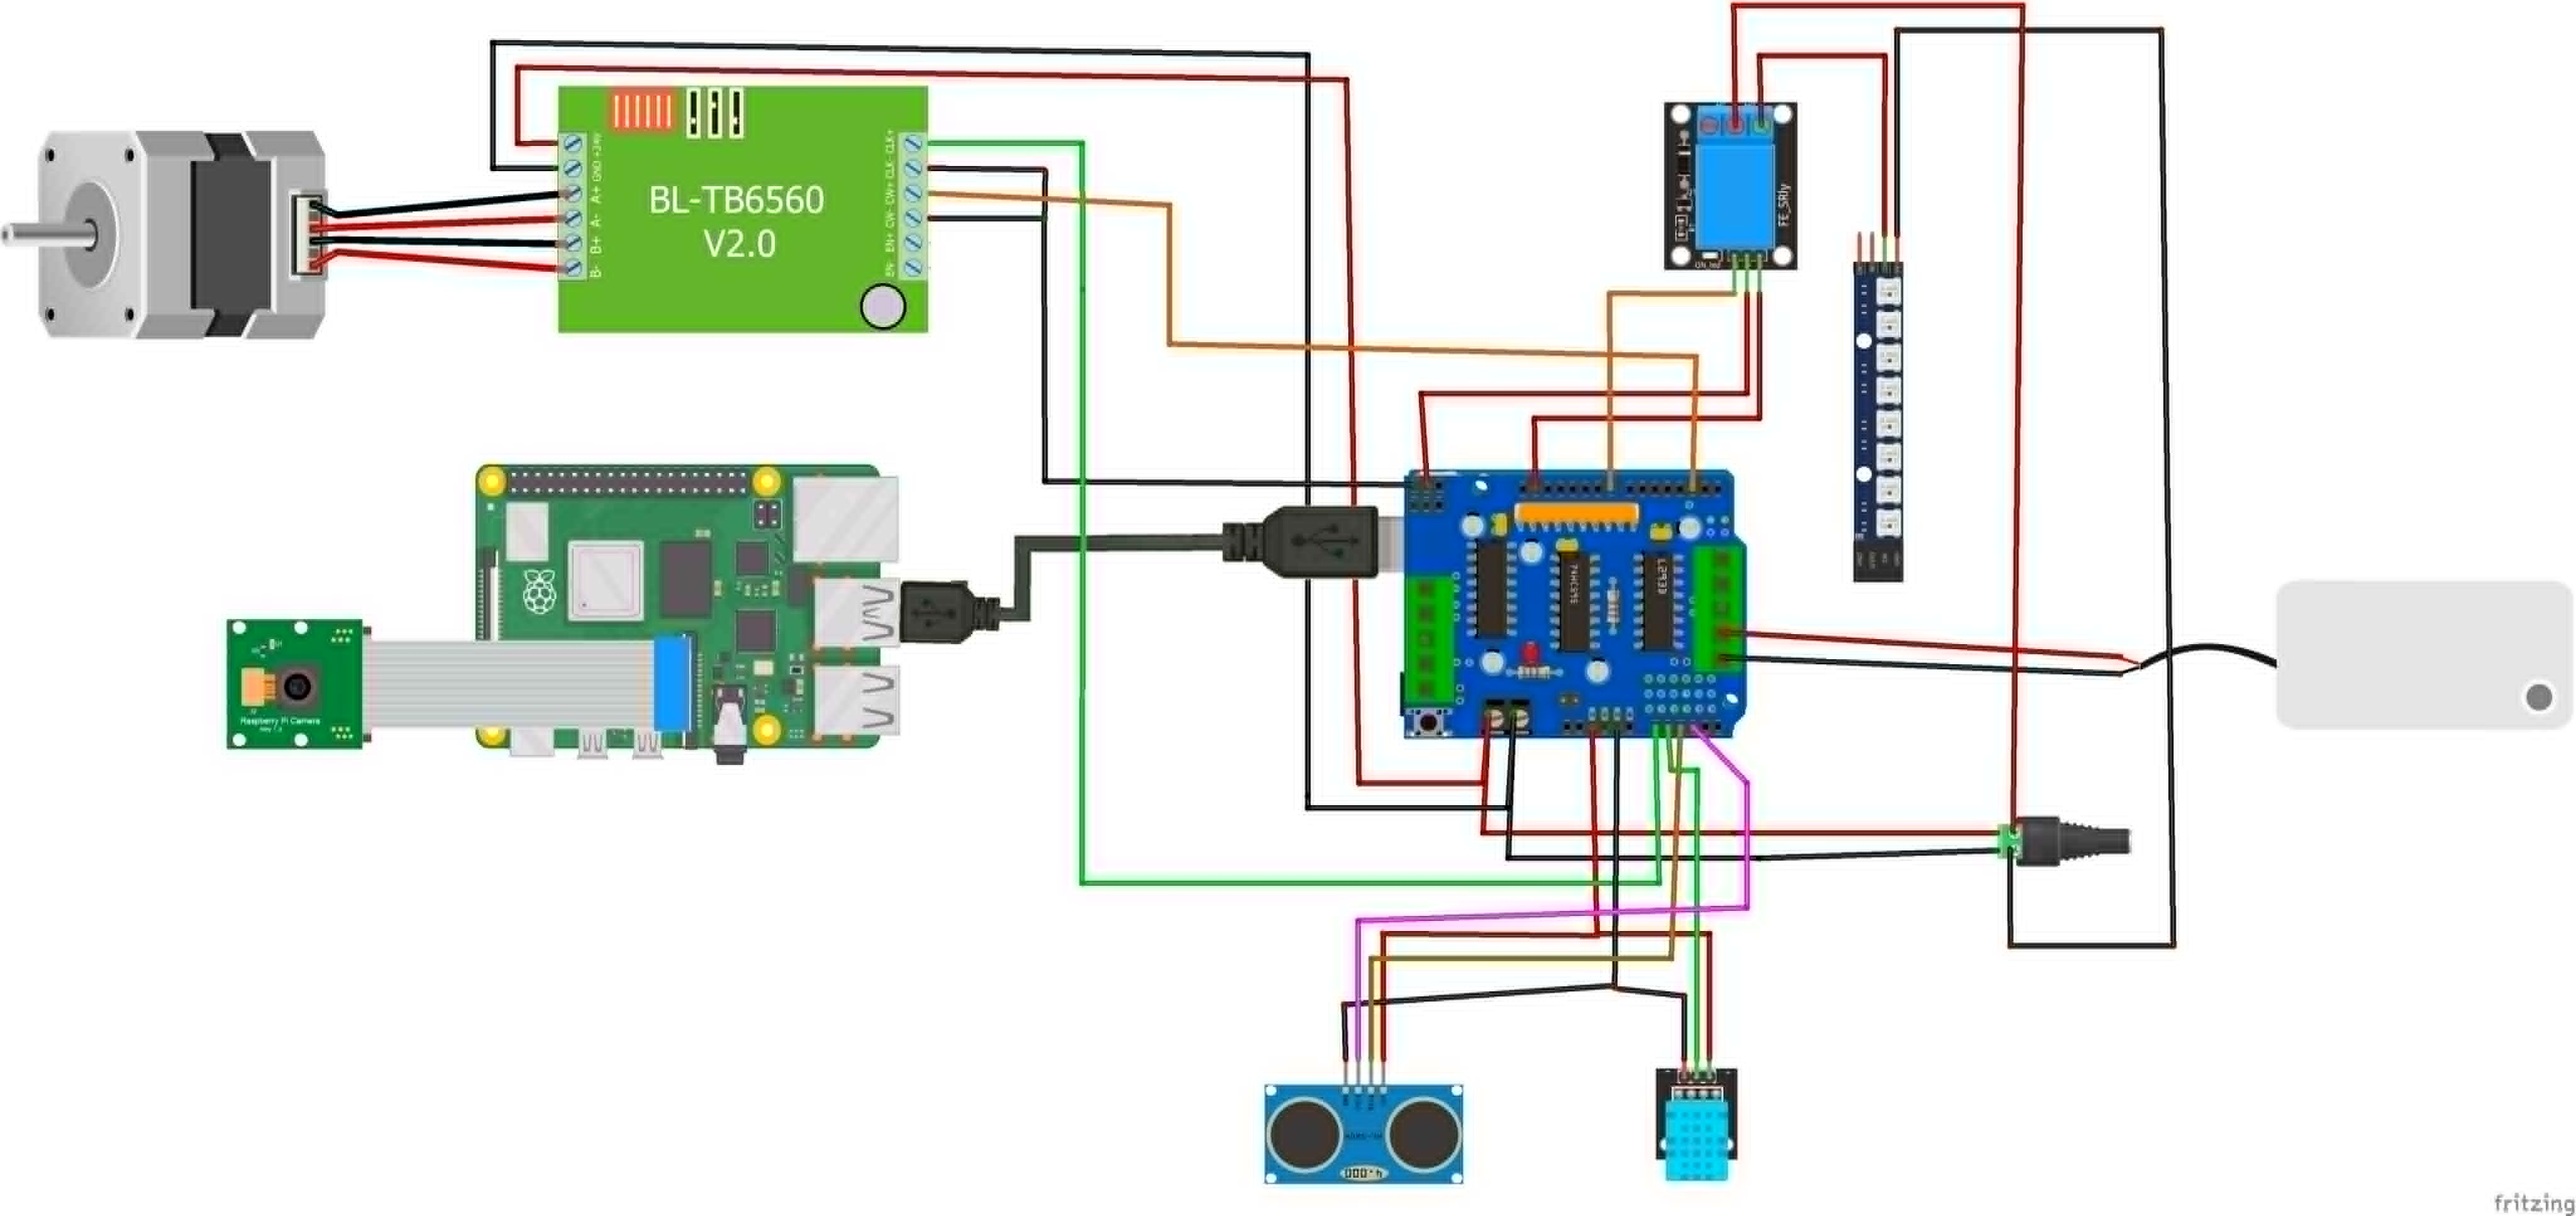
\includegraphics[width=0.7\linewidth]{public/cablage}
	\caption{Schéma détaillé du câblage des capteurs et actionneurs avec le microcontrôleur}
	\label{fig:cablage}
\end{figure}

La figure~\ref{fig:cablage} vient ainsi compléter la figure~\ref{fig:archi_iot} en apportant une vue détaillée de l’implémentation matérielle, depuis l’architecture globale jusqu’au niveau des connexions physiques.

\subsubsection*{Architecture logicielle embarquée}
La couche embarquée n'est pas figée : le logiciel exécuté sur le contrôleur est entièrement \textbf{versionné et mis à jour à distance} (voir la section~\ref{subsec:ota_thingsboard} consacrée à l'OTA). Sur le plan logiciel, le système embarqué se décompose en \textbf{deux ensembles complémentaires} :

\begin{itemize}
	\item \textbf{Le composant principal (« Main ») :} il regroupe le \textit{logiciel} déployé sur le Raspberry~Pi~4 et le \textit{micrologiciel} (\textit{firmware}) déployé sur l'Arduino. Le logiciel constitue le cœur applicatif du contrôleur : il établit et maintient la connexion MQTT avec le backend, dialogue avec le module d'intelligence artificielle et traduit les consignes reçues en commandes transmises au micrologiciel. Le micrologiciel, quant à lui, exécute de manière déterministe les tâches matérielles de proximité (acquisition des capteurs et pilotage des actionneurs).
	\item \textbf{Le service ThingsBoard (agent de déploiement) :} il s'agit d'un service autonome dont l'unique vocation est d'\textit{installer, surveiller et mettre à jour} le composant principal (logiciel et micrologiciel). Il assure l'enregistrement du contrôleur auprès de la plateforme ThingsBoard et orchestre l'application des mises à jour distantes (OTA), garantissant ainsi que la serre exécute toujours la dernière version validée du logiciel.
\end{itemize}
\begin{figure}[!htbp]
	\centering
	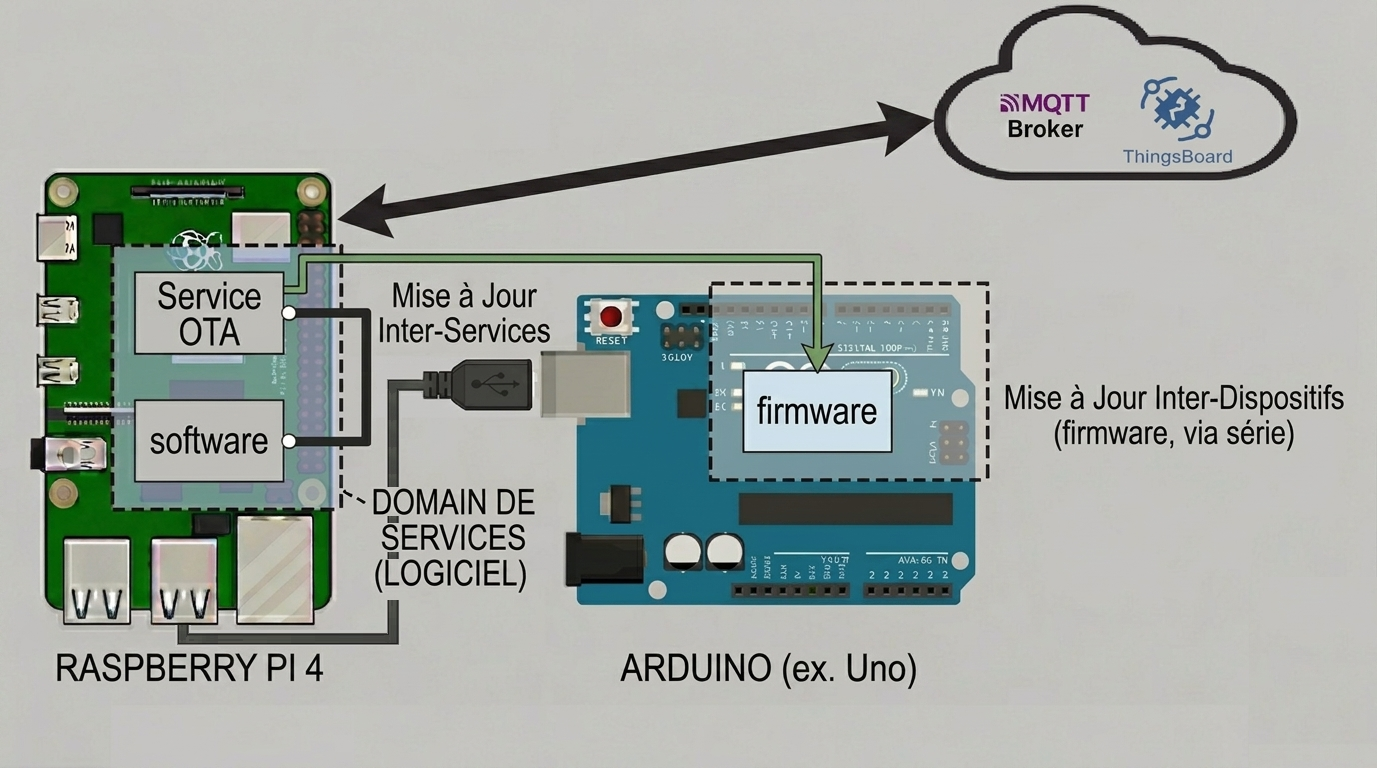
\includegraphics[width=0.7\linewidth]{public/relationLogEmbeded}
	\caption{Relation entre le composant principal et le service de déploiement ThingsBoard}
	\label{fig:relation_log_embedded}
\end{figure}
\paragraph{Architecture au sein du Raspberry Pi 4}
Le Raspberry Pi 4 constitue l'unité de coordination du système embarqué. Il héberge le logiciel principal (services de supervision, de communication et d'orchestration des traitements locaux) ainsi que l'agent de déploiement ThingsBoard. Son rôle principal est de centraliser les échanges avec le backend via MQTT, de dialoguer avec le module IA et de piloter la logique globale de la serre en relayant les commandes vers l'Arduino.

\begin{figure}[!htbp]
	\centering
	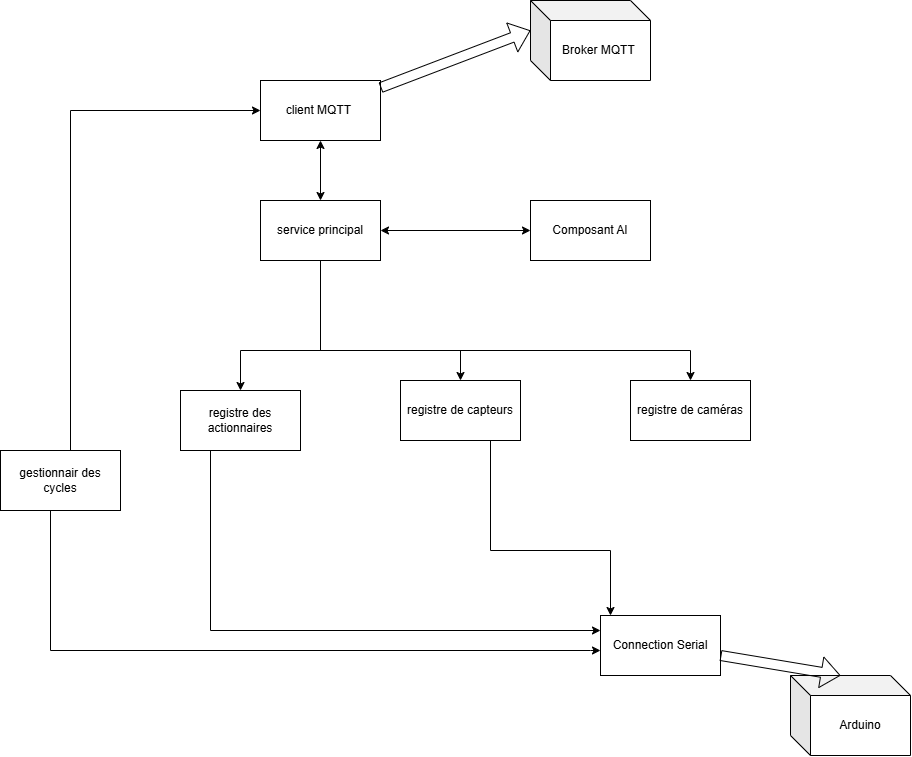
\includegraphics[width=0.9\linewidth]{public/raspiArchiDiagFR.png}
	\caption{Architecture logicielle embarquée au sein du système}
	\label{fig:embeededsoft}
\end{figure}

\paragraph{Architecture au sein de l'Arduino}
L'Arduino est dédié à l'exécution déterministe des tâches matérielles de proximité. Il prend en charge la lecture périodique des capteurs, la commande des actionneurs et l'application des consignes envoyées par le Raspberry Pi 4 via une liaison série. Cette séparation permet de conserver un comportement stable pour les opérations temps réel tout en réservant au Raspberry Pi les fonctions de communication.

L'implémentation du firmware embarqué a été confrontée à une contrainte importante liée aux ressources matérielles limitées de l'Arduino Uno, qui ne dispose que de 2 Ko de mémoire SRAM. Dans ce contexte, une architecture orientée objet classique basée sur l'héritage, le polymorphisme et l'instanciation de nombreuses classes aurait entraîné une consommation mémoire significative dès le démarrage du système.

Afin de garantir la compatibilité avec les ressources disponibles tout en conservant une architecture modulaire et extensible, une approche alternative a été adoptée. Celle-ci repose sur l'utilisation de structures légères associées à des pointeurs de fonctions permettant de représenter les différents périphériques de manière générique sans recourir à une hiérarchie complexe de classes.

Cette stratégie présente plusieurs avantages. D'une part, elle réduit considérablement l'occupation mémoire en supprimant les surcoûts associés aux mécanismes orientés objet traditionnels. D'autre part, elle permet d'ajouter de nouveaux périphériques en définissant uniquement les données spécifiques et les opérations nécessaires à leur fonctionnement. Enfin, l'ensemble des équipements peut être géré à travers une interface commune tout en conservant une empreinte mémoire compatible avec les contraintes du microcontrôleur.

Cette optimisation a permis d'intégrer simultanément plusieurs capteurs et actionneurs au sein du même firmware tout en préservant suffisamment de mémoire pour les buffers de communication série, les bibliothèques matérielles et les traitements temps réel nécessaires au fonctionnement de la serre intelligente.


Cette répartition des responsabilités garantit une architecture plus robuste : le Raspberry Pi 4 concentre les services applicatifs et intelligents, tandis que l'Arduino reste responsable du contrôle matériel de bas niveau.
\subsubsection*{Structure des messages série (Raspberry Pi \texorpdfstring{$\leftrightarrow$}{<->} Arduino)}
La communication entre le Raspberry Pi 4 et l'Arduino repose sur une liaison série UART utilisant un protocole de messages textuels structurés. Cette approche permet de simplifier le décodage des commandes tout en garantissant la lisibilité et la maintenabilité des échanges.

Les commandes envoyées par le Raspberry Pi respectent le format général suivant :


\texttt{<nom\_equipement>:<action>:<parametre\_1>:<parametre\_2>:...}


où :

\begin{itemize}
	\item \texttt{<nom\_equipement>} identifie le périphérique concerné ;
	\item \texttt{} représente l'opération à exécuter ;
	\item \texttt{<parametre\_i>} correspond aux paramètres associés à cette opération.
\end{itemize}

Par exemple, la commande :


\texttt{dc1:SPEED:200}


ordonne au moteur \texttt{dc1} de fonctionner à une vitesse de \texttt{200}.

Les réponses générées par l'Arduino utilisent quant à elles l'un des formats suivants :


\texttt{OK:value}


ou


\texttt{ERR:message}


Le premier indique l'exécution correcte de la commande tandis que le second signale une erreur détectée lors du traitement , par example : \texttt{OK:done} , \texttt{ERR:bad\_action}

\subsubsection*{Sécurité des communications IoT (MQTTS et TLS)}
Étant donné la nature critique des commandes transitant entre le Backend et la serre (ex: pilotage des pompes et vannes d'irrigation), la sécurité réseau est une composante structurelle de l'architecture. Toutes les communications télémétriques entre l'unité \textit{Edge} (Raspberry Pi 4) et le broker Mosquitto sont encapsulées dans un tunnel crypté utilisant le protocole \textbf{MQTTS} (MQTT sur TLS 1.2+). L'authentification mutuelle est assurée par l'échange de certificats X.509 et de clés asymétriques, prévenant ainsi toute attaque de type \textit{Man-in-the-Middle} (MitM) ou l'injection de fausses commandes matérielles. De plus, aucun secret critique (mot de passe base de données, clé d'API Gemini) n'est stocké en clair sur le dispositif physique local.

\subsubsection*{Mode Autonome (Architecture Offline-First)}
Conçu selon le paradigme \textit{Offline-First}, le contrôleur conserve une autonomie de fonctionnement complète en cas de coupure réseau : les cycles d'irrigation, d'éclairage et de ventilation sont maintenus localement à partir de la dernière configuration valide, tandis que les relevés non transmis sont temporisés dans un tampon local (SQLite) avant d'être resynchronisés avec le backend dès le rétablissement de la connexion.

\subsection{Le mécanisme d'attention et les Transformers}
Introduit pour le traitement automatique des langues~\cite{vaswani2017attention}, le mécanisme d'\textbf{auto-attention} permet à chaque élément d'une séquence d'interagir directement avec tous les autres, contrairement aux CNN qui ont une vision locale. Cette capacité à capturer des dépendances à longue distance est particulièrement utile en agriculture pour relier des symptômes distants sur une même plante. Les Transformers sont gourmands en données et en calcul, mais des variantes comme le \textbf{Swin Transformer}~\cite{liu2021swin} réduisent la complexité en limitant l'attention à des fenêtres locales.

\subsection{Grands modèles de langage (LLM)}
Les LLM (GPT, Gemini, etc.) sont des Transformers de type décodeur entraînés sur des masses de texte. Ils excellent en raisonnement et en génération de texte, mais sont \textbf{aveugles} : ils ne peuvent analyser une image. Pour le diagnostic agricole, ils doivent être combinés à un encodeur visuel.

\subsection{Modèles vision-langage (VLM)}
Un VLM associe trois composants : (1) un encodeur visuel (souvent un Vision Transformer), (2) un module d'alignement (projecteur ou Q-Former), (3) un LLM qui reçoit à la fois les tokens visuels et la question textuelle. Le tableau~\ref{tab:vlm_models} résume l'évolution récente.

\begin{table}[htbp]
	\centering
	\small
	\begin{tabularx}{\textwidth}{|l|c|Y|}
		\hline
		\rowcolor[HTML]{2C3E50}
		\textcolor{white}{\textbf{Modèle}} & \textcolor{white}{\textbf{Année}} & \textcolor{white}{\textbf{Innovation}} \\ \hline
		CLIP~\cite{radford2021learning} & 2021 & Apprentissage contrastif image-texte. \\
		BLIP-2~\cite{li2023blip2} & 2023 & Q-Former pour aligner vision et langage. \\
		LLaVA~\cite{liu2023llava} & 2023 & Projection linéaire + réglage par instructions. \\
		InstructBLIP~\cite{dai2023instructblip} & 2023 & Conditionnement du Q-Former par la question. \\
		\textbf{PaliGemma}~\cite{beyer2024paligemma} & 2024 & Architecture unifiée SigLIP + Gemma 2B. \\ \hline
	\end{tabularx}
	\caption{Évolution des modèles vision-langage}
	\label{tab:vlm_models}
\end{table}

La \textbf{question-réponse visuelle (VQA)} concrétise l'usage des VLM : l'utilisateur interroge le système en langage naturel, et le modèle répond en décrivant les symptômes (figure~\ref{fig:vqa-architecture}). Les VQA offrent une interaction guidée et une explicabilité, mais souffrent encore d'hallucinations, d'une forte dépendance au cloud, et d'une sensibilité aux conditions de prise de vue.

\begin{figure}[tbph]
	\centering
	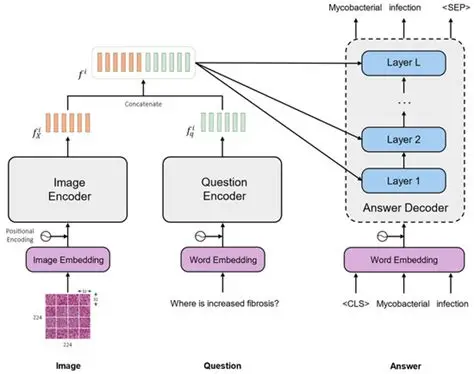
\includegraphics[width=0.7\linewidth]{public/vqa-architecture}
	\caption{Architecture fonctionnelle d'un système VQA.}
	\label{fig:vqa-architecture}
\end{figure}

\begin{figure}[tbph]
	\centering
	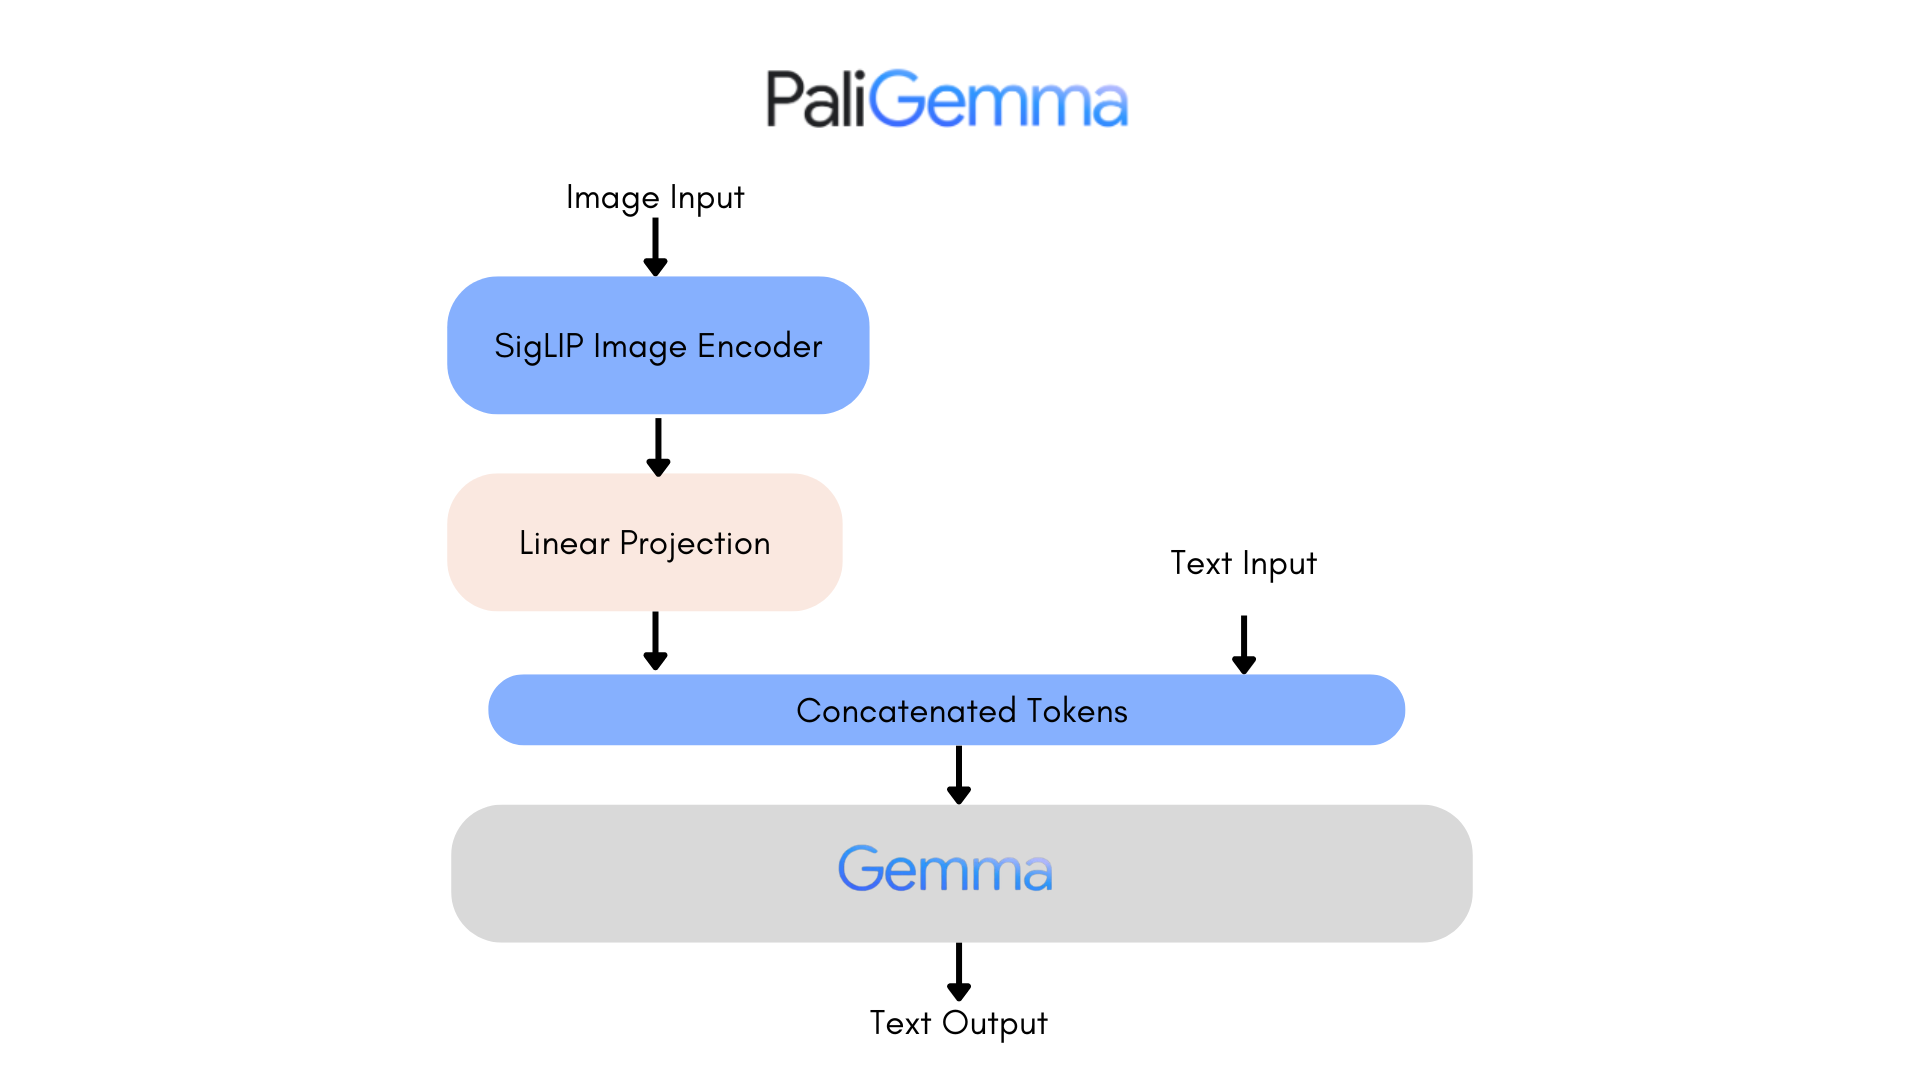
\includegraphics[width=0.7\linewidth]{public/paligemma_arch}
	\caption{Architecture de PaliGemma (SigLIP + Gemma).}
	\label{fig:paligemmaarch}
\end{figure}

% ============================================================

% ============================================================
\section{Apprentissage adaptatif et dynamique}
\label{sec:adaptive_dynamic}

L’agriculture de précision impose des modèles capables de s’adapter à des conditions changeantes (nouvelles maladies, variétés de plantes, environnements) tout en restant robustes et explicables. Cette section explore les techniques d’apprentissage qui permettent cette adaptabilité : les méthodes ensemblistes, l’apprentissage avec peu d’exemples (few-shot) et avec zéro exemple (zero-shot), ainsi que la sélection dynamique d’ensemble.

\subsection{Apprentissage par ensembles}
Les méthodes d’ensemble classiques, comme le \textit{bagging} (forêts aléatoires) ou le \textit{boosting} (AdaBoost, XGBoost), combinent plusieurs classifieurs pour réduire la variance et le biais. Appliquées aux réseaux de neurones, elles améliorent la robustesse : un ensemble de CNN peut surpasser n’importe lequel de ses membres pris isolément~\cite{dietterich2000ensemble}. Cependant, ces approches restent \textbf{statiques} : la combinaison des modèles est figée une fois l’entraînement terminé. Or, un modèle peut exceller sur certaines régions de l’espace des caractéristiques et être médiocre sur d’autres.

\subsection{Apprentissage avec peu d’exemples (few-shot)}
En environnement agricole réel, il est fréquent de devoir identifier une nouvelle maladie ou une variété végétale pour laquelle on ne dispose que de très peu d’images (parfois moins d’une dizaine). L’\textbf{apprentissage avec peu d’exemples} (few-shot learning) répond à ce besoin. Le \textbf{méta-apprentissage} (\textit{learning to learn}) en est une approche phare : l’algorithme MAML~\cite{finn2017model} apprend une initialisation des paramètres telle qu’une ou deux étapes de descente de gradient suffisent à adapter le modèle à une nouvelle tâche avec très peu de données. Cette capacité est cruciale pour un système comme HydroNova, qui doit pouvoir évoluer avec l’apparition de nouveaux pathogènes. D'autres approches comme \textit{Prototypical Networks}~\cite{snell2017prototypical} ou \textit{Relation Networks}~\cite{sung2018learning} sont également utilisées en agriculture~\cite{arguello2020few}.

\subsection{Apprentissage avec zéro exemple (zero-shot)}
Dans certains cas, aucune image de la nouvelle maladie n’est disponible au moment de l’entraînement. L’\textbf{apprentissage avec zéro exemple} (zero-shot learning) exploite des descriptions sémantiques (textuelles) des classes cibles. Les modèles vision-langage (VLM) comme CLIP~\cite{radford2021learning} ou PaliGemma sont naturellement adaptés au zero-shot : ils comparent l’image à une description textuelle de la maladie (par exemple, \textit{« taches brunes entourées d’un halo jaune sur feuilles de tomate »}) sans avoir jamais vu d’exemple visuel de cette pathologie. Cette approche est particulièrement pertinente pour les émergences phytosanitaires rapides~\cite{li2020zero}.

\subsection{Sélection dynamique d’ensemble (DES)}
Pour pallier le caractère statique des ensembles classiques, la \textbf{sélection dynamique d’ensemble} (DES) choisit, pour chaque image à classer, les modèles les plus compétents localement. Le framework \textbf{META-DES}~\cite{cruz2018meta} procède ainsi :
\begin{enumerate}
	\item Définition d’un voisinage de l’image cible (ses plus proches voisins dans un ensemble de validation).
	\item Extraction de \textit{méta-caractéristiques} pour chaque modèle candidat (précision locale, niveau de confiance, etc.).
	\item Prédiction par un méta-classifieur de la compétence du modèle pour cette image.
	\item Vote pondéré des seuls modèles jugés compétents.
\end{enumerate}
Cette approche améliore significativement la précision et la robustesse, particulièrement utile en milieu agricole où les conditions d’acquisition (éclairage, angle, chevauchement) varient fortement. Des travaux récents l'appliquent au diagnostic de maladies des plantes~\cite{zhang2020dynamic}.

\subsection{Pertinence dans le contexte agricole}
L’apprentissage adaptatif et dynamique répond à plusieurs contraintes du projet HydroNova :
\begin{itemize}
	\item \textbf{Évolutivité} : l’apparition de nouvelles maladies ou de nouvelles variétés de plantes peut être prise en compte via le few-shot ou le zero-shot, sans réentraînement complet.
	\item \textbf{Robustesse aux variations} : la sélection dynamique d’ensemble permet de s’adapter localement à des conditions de terrain changeantes.
	\item \textbf{Hybridation Edge/Cloud} : le few-shot et le zero-shot peuvent être déployés en cloud (via VLM), tandis que la sélection dynamique d’ensemble peut être embarquée sur le Raspberry Pi pour une inférence rapide hors-ligne.
\end{itemize}
Ces techniques complètent ainsi naturellement l’architecture hybride proposée : le module embarqué repose sur un ensemble dynamique de CNN (DES), tandis que le module cloud exploite un VLM capable de zero-shot et de few-shot.

% ============================================================
\section{Synthèse critique et positionnement}
\label{sec:synthese}

Le tableau~\ref{tab:synthese} compare les différentes familles de modèles selon des critères opérationnels.

\begin{table}[htbp]
	\centering
	\small
	\begin{tabularx}{\textwidth}{|l|X|X|c|c|}
		\hline
		\rowcolor[HTML]{2C3E50}
		\textcolor{white}{\textbf{Approche}} & \textcolor{white}{\textbf{Apports}} & \textcolor{white}{\textbf{Limites}} & \textcolor{white}{\textbf{Offline}} & \textcolor{white}{\textbf{Explicabilité}} \\ \hline
		CNN classiques & Efficaces, légers & Fragiles, boîtes noires & Oui & Faible \\
		Ensembles de CNN & Robustesse & Complexité & Oui & Faible/Moyenne \\
		Vision Transformers & Modélisation globale & Gourmands & Partiel & Moyenne \\
		LLM & Raisonnement, texte & Aveugles & Non & Élevée \\
		VLM / VQA & Multimodal, explicatif & Hallucinations, dépendance cloud & Non & Élevée \\
		Few-shot / Zero-shot & Adaptabilité rapide & Nécessite un pré-entraînement adapté & Partiel & Moyenne/Élevée \\
		DES (sélection dynamique) & Robustesse locale & Coût de calcul supplémentaire & Oui & Moyenne \\ \hline
	\end{tabularx}
	\caption{Synthèse comparative des paradigmes d'IA pour le diagnostic agricole}
	\label{tab:synthese}
\end{table}

Aucune approche unique ne satisfait toutes les contraintes du projet HydroNova : besoin d'un fonctionnement hors-ligne (serres isolées), de robustesse aux conditions réelles, d'évolutivité face à de nouvelles maladies, et d'explicabilité pour l'utilisateur.

C'est pourquoi nous proposons une \textbf{architecture hybride} articulant deux branches complémentaires :

\begin{itemize}
	\item Une branche \textbf{Edge} (embarquée sur Raspberry Pi) basée sur un ensemble dynamique de CNN (META-DES) pour une classification robuste, rapide et hors-ligne.
	\item Une branche \textbf{Cloud} exploitant un VLM (PaliGemma) pour l'assistance interactive, la génération d'explications, les cas ambigus, ainsi que l'adaptation en cas d'absence d'exemples.
\end{itemize}

Cette hybridation permet de concilier performance, résilience, adaptabilité et richesse sémantique.

% ============================================================
\section*{Conclusion}
\addcontentsline{toc}{section}{Conclusion}

Ce chapitre a présenté un panorama des principales architectures d'intelligence artificielle pour l'agriculture : CNN, Transformers, VLM, ainsi que les techniques d'apprentissage adaptatif et dynamique (ensembles, few-shot, zero-shot, sélection dynamique). L'analyse montre qu'aucun modèle isolé n'est suffisant, ce qui justifie l'approche hybride d'HydroNova. Le chapitre suivant détaille l'analyse des besoins et la spécification fonctionnelle du système.
\include{Chapitre5}
% ============================================================
% CHAPITRE II — ÉTAT DE L'ART
% ============================================================
\chapter{ÉTAT DE L'ART : APPROCHES INTELLIGENTES EN AGRICULTURE}

\section*{Introduction}
\addcontentsline{toc}{section}{Introduction}

L'agriculture moderne est confrontée à un double défi : augmenter les rendements tout en réduisant l'impact environnemental. En Tunisie, les pertes dues aux maladies végétales sont estimées entre 20\,\% et 40\,\% des récoltes~\cite{fao2021report}. L'absence d'outils de diagnostic précoce et accessible sur le terrain aggrave cette situation. L'intelligence artificielle, en particulier l'apprentissage profond appliqué à la vision par ordinateur et au traitement du langage naturel, ouvre des perspectives prometteuses.


Ce chapitre dresse un panorama critique des principales familles de modèles utilisables pour la détection des maladies végétales et l'assistance agricole. La première section présente les réseaux de neurones convolutifs (CNN), leur fonctionnement, leur évolution et leurs limites en conditions réelles. La deuxième section aborde les Transformers et les modèles vision-langage (VLM), qui intègrent des mécanismes d'attention et permettent l'interaction multimodale. La troisième section explore les techniques d'apprentissage adaptatif et dynamique: ensembles, few-shot, zero-shot et sélection dynamique, qui répondent aux contraintes d'évolutivité, de robustesse et d'hybridation Edge/Cloud. Une synthèse critique et le positionnement de l'architecture retenue pour le projet HydroNova concluent le chapitre.
\newpage
% ============================================================
\section{Réseaux de neurones convolutifs (CNN)}
\label{sec:cnnn}

\subsection{Principe général}
Les réseaux de neurones convolutifs (CNN) ont été conçus pour traiter efficacement des données structurées en grille, comme les images. Contrairement aux réseaux entièrement connectés, ils exploitent deux idées clés :

\begin{itemize}
	\item \textbf{Convolutions locales} : chaque neurone ne regarde qu'une petite région de l'image (son champ récepteur), ce qui réduit drastiquement le nombre de paramètres.
	\item \textbf{Partage des poids} : le même filtre (ou noyau) est appliqué sur toute l'image, ce qui rend le modèle invariant aux translations (un motif pathologique est reconnu où qu'il se trouve).
\end{itemize}

Une couche de convolution produit une \textit{carte de caractéristiques} (\textit{feature map}) qui met en évidence la présence de motifs élémentaires (contours, textures, taches). En empilant plusieurs couches, le modèle apprend des représentations de plus en plus abstraites : des arêtes dans les premières couches jusqu'aux structures sémantiques complexes (nécroses, lésions) dans les couches profondes. Des couches de \textit{pooling} (sous-échantillonnage) introduisent une certaine invariance aux petites déformations.


\subsection{Évolution des architectures CNN}
Le tableau~\ref{tab:cnn_archi} retrace les grandes étapes de l'évolution des CNN.

\begin{table}[htbp]
	\centering
	\small
	\begin{tabularx}{\textwidth}{|l|c|c|Y|}
		\hline
		\rowcolor[HTML]{2C3E50}
		\textcolor{white}{\textbf{Architecture}} & \textcolor{white}{\textbf{Année}} & \textcolor{white}{\textbf{ImageNet Top-1}} & \textcolor{white}{\textbf{Innovation clé}} \\ \hline
		AlexNet~\cite{krizhevsky2012imagenet} & 2012 & 63,3\,\% & ReLU, Dropout, parallélisation GPU. \\
		VGGNet-16~\cite{simonyan2014very} & 2014 & 74,4\,\% & Empilement de petits filtres 3×3. \\
		GoogLeNet~\cite{szegedy2015going} & 2015 & 74,8\,\% & Modules Inception (convolutions multi-échelles). \\
		ResNet-50~\cite{he2016deep} & 2016 & 76,1\,\% & Connexions résiduelles (\textit{skip connections}). \\
		InceptionV3~\cite{szegedy2016rethinking} & 2016 & 77,9\,\% & Factorisation des noyaux. \\
		MobileNetV2~\cite{howard2017mobilenets} & 2017 & 72,0\,\% & Convolutions séparables en profondeur (embarqué). \\
		EfficientNet-B4~\cite{tan2019efficientnet} & 2019 & 83,0\,\% & Mise à l'échelle coordonnée. \\
		ConvNeXt-T~\cite{liu2022convnet} & 2022 & 82,1\,\% & Modernisation inspirée des Transformers. \\ \hline
	\end{tabularx}
	\caption{Évolution des architectures CNN de référence}
	\label{tab:cnn_archi}
\end{table}

Les figures~\ref{fig:architecture-of-the-inceptionv3}, \ref{fig:ResNet-architecture} et \ref{fig:architecture-of-the-convnext} illustrent respectivement InceptionV3, ResNet et ConvNeXt.

\begin{figure}[h!]
	\centering
	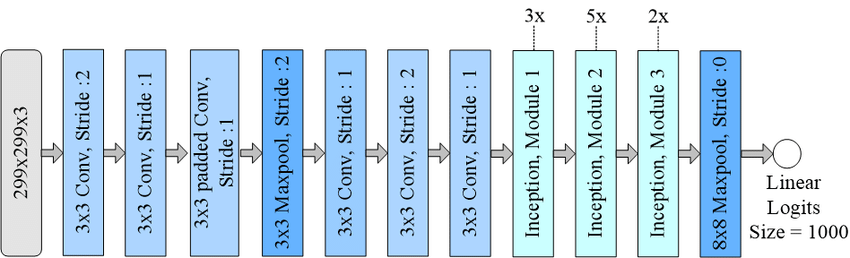
\includegraphics[width=0.7\linewidth]{public/Architecture-of-the-InceptionV3}
	\caption{Architecture d'InceptionV3 avec ses blocs parallèles.}
	\label{fig:architecture-of-the-inceptionv3}
\end{figure}

\begin{figure}[h!]
	\centering
	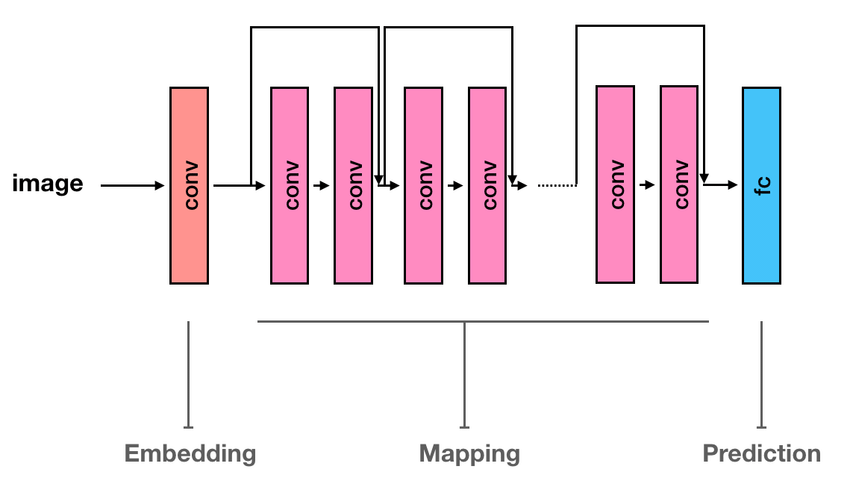
\includegraphics[width=0.7\linewidth]{public/resnetArchi}
	\caption{Architecture de ResNet (connexions résiduelles).}
	\label{fig:ResNet-architecture}
\end{figure}

\begin{figure}[h!]
	\centering
	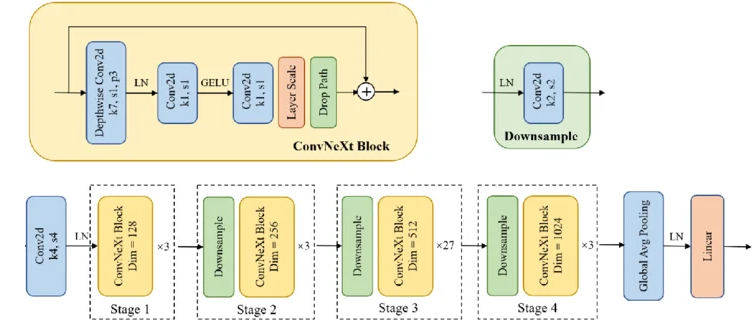
\includegraphics[width=0.7\linewidth]{public/Architecture-of-the-ConvNeXt}
	\caption{Architecture de ConvNeXt.}
	\label{fig:architecture-of-the-convnext}
\end{figure}
\newpage
\subsection{Limites des CNN pour le diagnostic agricole}
Les CNNs ont montré leur efficacité pour la classification de maladies sur des jeux de données comme \textit{PlantVillage}. Mohanty et al.~\cite{mohanty2016using} ont atteint une précision de 99,35\,\% pour 26 maladies sur 14 espèces. Too et al.~\cite{too2019comparative} ont comparé plusieurs architectures (VGG, ResNet, DenseNet) et conclu que les réseaux avec connexions résiduelles ou denses offrent une meilleure stabilité.

Cependant, des limites importantes apparaissent dès que l'on sort du cadre contrôlé du laboratoire~\cite{barbedo2018factors} :

\begin{enumerate}
	\item \textbf{Manque d'explicabilité} : un CNN donne une probabilité, mais ne peut expliquer son raisonnement (par exemple, sur quels pixels il s'appuie).
	\item \textbf{Information unidirectionnelle} : impossible d'intégrer des données contextuelles (historique de la culture, conditions climatiques) ou des questions de l'utilisateur.
	\item \textbf{Fragilité aux variations réelles} : changement d'éclairage, flou de bougé, chevauchement de feuilles dégradent fortement les performances.
\end{enumerate}

Ces lacunes motivent l'exploration d'architectures plus récentes, basées sur l'attention et la multimodalité.
% ============================================================
\section{Transformers et modèles vision-langage}
\label{sec:transformer_vlm}

\subsection{Le mécanisme d'attention et les Transformers}
Introduit pour le traitement automatique des langues~\cite{vaswani2017attention}, le mécanisme d'\textbf{auto-attention} permet à chaque élément d'une séquence d'interagir directement avec tous les autres, contrairement aux CNN qui ont une vision locale. Cette capacité à capturer des dépendances à longue distance est particulièrement utile en agriculture pour relier des symptômes distants sur une même plante. Les Transformers sont gourmands en données et en calcul, mais des variantes comme le \textbf{Swin Transformer}~\cite{liu2021swin} réduisent la complexité en limitant l'attention à des fenêtres locales.

\subsection{Grands modèles de langage (LLM)}
Les LLM (GPT, Gemini, etc.) sont des Transformers de type décodeur entraînés sur des masses de texte. Ils excellent en raisonnement et en génération de texte, mais sont \textbf{aveugles} : ils ne peuvent analyser une image. Pour le diagnostic agricole, ils doivent être combinés à un encodeur visuel.

\subsection{Modèles vision-langage (VLM)}
Un VLM associe trois composants : (1) un encodeur visuel (souvent un Vision Transformer), (2) un module d'alignement (projecteur ou Q-Former), (3) un LLM qui reçoit à la fois les tokens visuels et la question textuelle. Le tableau~\ref{tab:vlm_models} résume l'évolution récente.

\begin{table}[htbp]
	\centering
	\small
	\begin{tabularx}{\textwidth}{|l|c|Y|}
		\hline
		\rowcolor[HTML]{2C3E50}
		\textcolor{white}{\textbf{Modèle}} & \textcolor{white}{\textbf{Année}} & \textcolor{white}{\textbf{Innovation}} \\ \hline
		CLIP~\cite{radford2021learning} & 2021 & Apprentissage contrastif image-texte. \\
		BLIP-2~\cite{li2023blip2} & 2023 & Q-Former pour aligner vision et langage. \\
		LLaVA~\cite{liu2023llava} & 2023 & Projection linéaire + réglage par instructions. \\
		InstructBLIP~\cite{dai2023instructblip} & 2023 & Conditionnement du Q-Former par la question. \\
		\textbf{PaliGemma}~\cite{beyer2024paligemma} & 2024 & Architecture unifiée SigLIP + Gemma 2B. \\ \hline
	\end{tabularx}
	\caption{Évolution des modèles vision-langage}
	\label{tab:vlm_models}
\end{table}

La \textbf{question-réponse visuelle (VQA)} concrétise l'usage des VLM : l'utilisateur interroge le système en langage naturel, et le modèle répond en décrivant les symptômes (figure~\ref{fig:vqa-architecture}). Les VQA offrent une interaction guidée et une explicabilité, mais souffrent encore d'hallucinations, d'une forte dépendance au cloud, et d'une sensibilité aux conditions de prise de vue.

\begin{figure}[tbph]
	\centering
	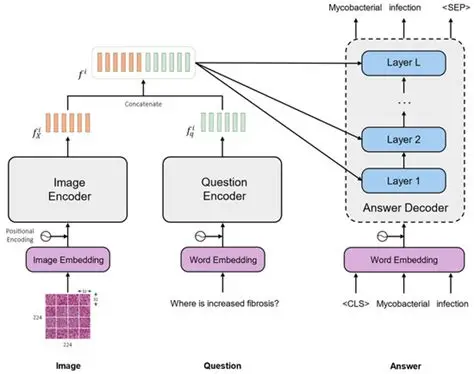
\includegraphics[width=0.7\linewidth]{public/vqa-architecture}
	\caption{Architecture fonctionnelle d'un système VQA.}
	\label{fig:vqa-architecture}
\end{figure}

\begin{figure}[tbph]
	\centering
	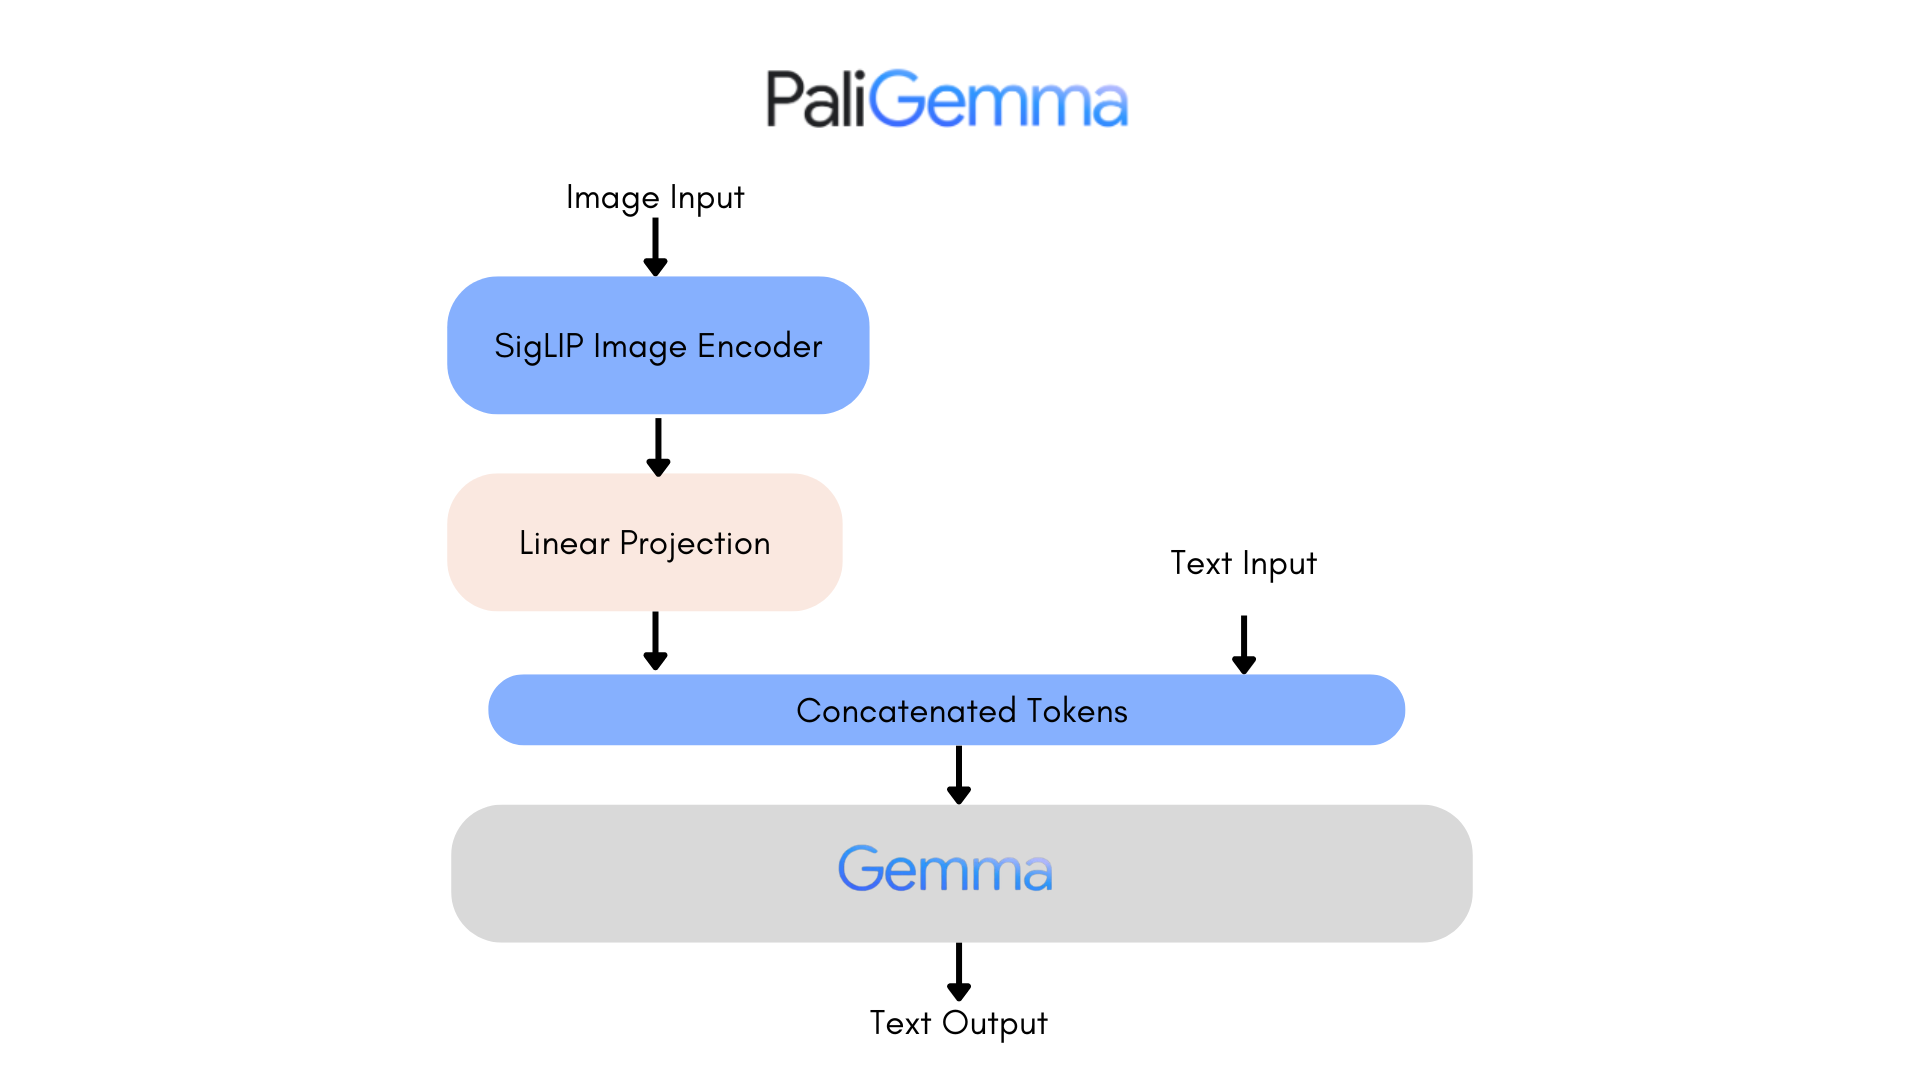
\includegraphics[width=0.7\linewidth]{public/paligemma_arch}
	\caption{Architecture de PaliGemma (SigLIP + Gemma).}
	\label{fig:paligemmaarch}
\end{figure}

% ============================================================

% ============================================================
\section{Apprentissage adaptatif et dynamique}
\label{sec:adaptive_dynamic}

L’agriculture de précision impose des modèles capables de s’adapter à des conditions changeantes (nouvelles maladies, variétés de plantes, environnements) tout en restant robustes et explicables. Cette section explore les techniques d’apprentissage qui permettent cette adaptabilité : les méthodes ensemblistes, l’apprentissage avec peu d’exemples (few-shot) et avec zéro exemple (zero-shot), ainsi que la sélection dynamique d’ensemble.

\subsection{Apprentissage par ensembles}
Les méthodes d’ensemble classiques, comme le \textit{bagging} (forêts aléatoires) ou le \textit{boosting} (AdaBoost, XGBoost), combinent plusieurs classifieurs pour réduire la variance et le biais. Appliquées aux réseaux de neurones, elles améliorent la robustesse : un ensemble de CNN peut surpasser n’importe lequel de ses membres pris isolément~\cite{dietterich2000ensemble}. Cependant, ces approches restent \textbf{statiques} : la combinaison des modèles est figée une fois l’entraînement terminé. Or, un modèle peut exceller sur certaines régions de l’espace des caractéristiques et être médiocre sur d’autres.

\subsection{Apprentissage avec peu d’exemples (few-shot)}
En environnement agricole réel, il est fréquent de devoir identifier une nouvelle maladie ou une variété végétale pour laquelle on ne dispose que de très peu d’images (parfois moins d’une dizaine). L’\textbf{apprentissage avec peu d’exemples} (few-shot learning) répond à ce besoin. Le \textbf{méta-apprentissage} (\textit{learning to learn}) en est une approche phare : l’algorithme MAML~\cite{finn2017model} apprend une initialisation des paramètres telle qu’une ou deux étapes de descente de gradient suffisent à adapter le modèle à une nouvelle tâche avec très peu de données. Cette capacité est cruciale pour un système comme HydroNova, qui doit pouvoir évoluer avec l’apparition de nouveaux pathogènes. D'autres approches comme \textit{Prototypical Networks}~\cite{snell2017prototypical} ou \textit{Relation Networks}~\cite{sung2018learning} sont également utilisées en agriculture~\cite{arguello2020few}.

\subsection{Apprentissage avec zéro exemple (zero-shot)}
Dans certains cas, aucune image de la nouvelle maladie n’est disponible au moment de l’entraînement. L’\textbf{apprentissage avec zéro exemple} (zero-shot learning) exploite des descriptions sémantiques (textuelles) des classes cibles. Les modèles vision-langage (VLM) comme CLIP~\cite{radford2021learning} ou PaliGemma sont naturellement adaptés au zero-shot : ils comparent l’image à une description textuelle de la maladie (par exemple, \textit{« taches brunes entourées d’un halo jaune sur feuilles de tomate »}) sans avoir jamais vu d’exemple visuel de cette pathologie. Cette approche est particulièrement pertinente pour les émergences phytosanitaires rapides~\cite{li2020zero}.

\subsection{Sélection dynamique d’ensemble (DES)}
Pour pallier le caractère statique des ensembles classiques, la \textbf{sélection dynamique d’ensemble} (DES) choisit, pour chaque image à classer, les modèles les plus compétents localement. Le framework \textbf{META-DES}~\cite{cruz2018meta} procède ainsi :
\begin{enumerate}
	\item Définition d’un voisinage de l’image cible (ses plus proches voisins dans un ensemble de validation).
	\item Extraction de \textit{méta-caractéristiques} pour chaque modèle candidat (précision locale, niveau de confiance, etc.).
	\item Prédiction par un méta-classifieur de la compétence du modèle pour cette image.
	\item Vote pondéré des seuls modèles jugés compétents.
\end{enumerate}
Cette approche améliore significativement la précision et la robustesse, particulièrement utile en milieu agricole où les conditions d’acquisition (éclairage, angle, chevauchement) varient fortement. Des travaux récents l'appliquent au diagnostic de maladies des plantes~\cite{zhang2020dynamic}.

\subsection{Pertinence dans le contexte agricole}
L’apprentissage adaptatif et dynamique répond à plusieurs contraintes du projet HydroNova :
\begin{itemize}
	\item \textbf{Évolutivité} : l’apparition de nouvelles maladies ou de nouvelles variétés de plantes peut être prise en compte via le few-shot ou le zero-shot, sans réentraînement complet.
	\item \textbf{Robustesse aux variations} : la sélection dynamique d’ensemble permet de s’adapter localement à des conditions de terrain changeantes.
	\item \textbf{Hybridation Edge/Cloud} : le few-shot et le zero-shot peuvent être déployés en cloud (via VLM), tandis que la sélection dynamique d’ensemble peut être embarquée sur le Raspberry Pi pour une inférence rapide hors-ligne.
\end{itemize}
Ces techniques complètent ainsi naturellement l’architecture hybride proposée : le module embarqué repose sur un ensemble dynamique de CNN (DES), tandis que le module cloud exploite un VLM capable de zero-shot et de few-shot.

% ============================================================
\section{Synthèse critique et positionnement}
\label{sec:synthese}

Le tableau~\ref{tab:synthese} compare les différentes familles de modèles selon des critères opérationnels.

\begin{table}[htbp]
	\centering
	\small
	\begin{tabularx}{\textwidth}{|l|X|X|c|c|}
		\hline
		\rowcolor[HTML]{2C3E50}
		\textcolor{white}{\textbf{Approche}} & \textcolor{white}{\textbf{Apports}} & \textcolor{white}{\textbf{Limites}} & \textcolor{white}{\textbf{Offline}} & \textcolor{white}{\textbf{Explicabilité}} \\ \hline
		CNN classiques & Efficaces, légers & Fragiles, boîtes noires & Oui & Faible \\
		Ensembles de CNN & Robustesse & Complexité & Oui & Faible/Moyenne \\
		Vision Transformers & Modélisation globale & Gourmands & Partiel & Moyenne \\
		LLM & Raisonnement, texte & Aveugles & Non & Élevée \\
		VLM / VQA & Multimodal, explicatif & Hallucinations, dépendance cloud & Non & Élevée \\
		Few-shot / Zero-shot & Adaptabilité rapide & Nécessite un pré-entraînement adapté & Partiel & Moyenne/Élevée \\
		DES (sélection dynamique) & Robustesse locale & Coût de calcul supplémentaire & Oui & Moyenne \\ \hline
	\end{tabularx}
	\caption{Synthèse comparative des paradigmes d'IA pour le diagnostic agricole}
	\label{tab:synthese}
\end{table}

Aucune approche unique ne satisfait toutes les contraintes du projet HydroNova : besoin d'un fonctionnement hors-ligne (serres isolées), de robustesse aux conditions réelles, d'évolutivité face à de nouvelles maladies, et d'explicabilité pour l'utilisateur.

C'est pourquoi nous proposons une \textbf{architecture hybride} articulant deux branches complémentaires :

\begin{itemize}
	\item Une branche \textbf{Edge} (embarquée sur Raspberry Pi) basée sur un ensemble dynamique de CNN (META-DES) pour une classification robuste, rapide et hors-ligne.
	\item Une branche \textbf{Cloud} exploitant un VLM (PaliGemma) pour l'assistance interactive, la génération d'explications, les cas ambigus, ainsi que l'adaptation en cas d'absence d'exemples.
\end{itemize}

Cette hybridation permet de concilier performance, résilience, adaptabilité et richesse sémantique.

% ============================================================
\section*{Conclusion}
\addcontentsline{toc}{section}{Conclusion}

Ce chapitre a présenté un panorama des principales architectures d'intelligence artificielle pour l'agriculture : CNN, Transformers, VLM, ainsi que les techniques d'apprentissage adaptatif et dynamique (ensembles, few-shot, zero-shot, sélection dynamique). L'analyse montre qu'aucun modèle isolé n'est suffisant, ce qui justifie l'approche hybride d'HydroNova. Le chapitre suivant détaille l'analyse des besoins et la spécification fonctionnelle du système.

\clearpage
%\chapter*{Bibliographie}
\addcontentsline{toc}{chapter}{Bibliographie}
\bibliographystyle{plain}
\bibliography{references}


\end{document}